\chapter{Cross-Population Robustness (RQ3)}
\label{ch:rq3}

\providecommand{\missingfigure}[1]{%
\fcolorbox{red}{white}{%
\parbox[c][0.14\textheight][c]{0.9\textwidth}{\centering\textcolor{red}{Placeholder figure\\\texttt{\detokenize{#1}}}}%
}%
}

\section{Motivation and Connection to RQ2}
\label{sec:rq3-motivation}

The dialect analysis in Chapter~\ref{ch:rq2} gave us a clear picture. When we train twenty PACE populations on Zipfian datasets that share the same concentration $\alpha$ but differ in which pairs are ranked at the top, the populations end up learning different abstraction libraries. The more concentrated the distribution, the more the libraries diverge. And by looking at individual cases at moderate $\alpha$, we could see why: the abstractions each population adopts trace back to the specific pairs that happen to be frequent in its dataset. Two populations trained on rankings that put different pairs at the top will therefore find themselves talking about different structural regularities.

This puts a natural question on the table. If each population's library is bound to its own top-ranked pairs, can two populations still communicate with each other? Consider a speaker that has learned during its training that a certain token in its message vocabulary should be produced when it wants to describe a certain substructure of its most frequent pair. A listener from a different population has, in general, learned no such association: its top-ranked pair was different, and so its message vocabulary carries different meanings. When the two are put in the same conversation, we should expect the speaker's messages to be misinterpreted, and the reconstruction of the target scene to suffer.

RQ3 breaks this general prediction into three concrete questions, ordered by how far each pushes the mismatch between the two agents. The first question is whether same-$\alpha$ populations already show measurable communication difficulties, even though they share the shape of their training distribution and only differ in which pairs sit at the top of the ranking. The second question is what happens when we make the mismatch larger, pairing agents that come from different $\alpha$ altogether, so that even the shape of their training distributions no longer matches. The third question is whether the same kind of breakdown appears not between two agents, but between a single agent and a distribution it never saw during training, so that the mismatch is between the agent and its environment.

Each question is addressed in a separate group of experiments. Section~\ref{sec:rq3-group-c} (Group C) reports the same-$\alpha$ cross-pairing experiments and asks whether we can detect a communication difficulty when the two agents come from the same $\alpha$ but from different rankings. Section~\ref{sec:rq3-group-m} (Group M) presents three modifications to that base setup, introduced along the way as we tried to understand what the bandit was actually doing during joint training. Section~\ref{sec:rq3-group-x} (Group X) moves to the cross-$\alpha$ setting, where the two agents come from different concentration parameters. Section~\ref{sec:rq3-group-o} (Group O) turns to two case studies in which the setup is pushed further out of training distribution: a mixed-distribution interaction and an out-of-distribution shift, together with a qualitative analysis of the single case that shows substantial dynamics on the bandit side. Section~\ref{sec:rq3-discussion} pulls the four groups together and returns to the connection with Chapter~\ref{ch:rq2}.

A brief remark on the labels we use for experiments. This chapter organises its experiments into four groups, each denoted by a letter that reflects what the group tests:

\begin{itemize}
    \item C: cross-pairing between agents that share $\alpha$ but differ in ranking;
    \item M: modifications to the same-$\alpha$ setup that let us look inside the adaptation mechanism;
    \item X: cross-$\alpha$ pairings between agents from different concentration parameters;
    \item O: out-of-training-distribution case studies, in which the agents interact under conditions further from those they were trained on.
\end{itemize}

Individual experiments within each group are then numbered (C1, C2, M3, and so on).

\section{Same-$\alpha$ Cross-Pairing (Group C)}
\label{sec:rq3-group-c}

\subsection{Experimental Design}
\label{sec:rq3-c-design}

For each of three representative $\alpha$ values, 0.60, 1.80, and 3.00, we take a fixed speaker and pair it with several listeners. The speaker is always the trained network of seed 42 at the given $\alpha$, and for the entire experiment we freeze both its neural weights and its bandit state. The listeners are trained networks of other seeds at the same $\alpha$, and they are the only agents allowed to adapt during joint training. We leave $\alpha = 0.00$ out of the design because at that concentration every seed produces the same uniform distribution by construction, and the notions of close, median, and far collapse.

For each $\alpha$ we run four pairings. One is a within-pairing baseline, in which the speaker is paired with its own original listener (both from seed 42). The other three are cross-pairings, in which the speaker is paired with listeners from three different seeds, chosen to span the range of distributional distance from the speaker. The within-pairing gives us an upper bound on how well the joint model can do at that $\alpha$, since it removes any mismatch between speaker and listener.

In each cross-pairing, we load the speaker network from its end-of-training checkpoint and freeze it, so that neither its weights nor its bandit Q-values change during joint training. We also load the speaker's bandit state, which means that the messages produced during joint training reflect the speaker's actual communication policy at the end of its own training, not a fresh policy with no abstractions in use. The listener starts from its own end-of-training checkpoint and adapts through gradient descent on the reconstruction loss.

Joint training runs for 20 epochs. We measure reconstruction accuracy on the speaker's held-out test set at epoch 0, before any training, and after every subsequent epoch. The epoch-0 measurement is important on its own: it tells us how well the two agents already understand each other without any adaptation, which is the most direct proxy for out-of-the-box compatibility. Later epochs tell us how quickly the listener adapts and what plateau it eventually reaches.

\subsection{Three Definitions of Distributional Distance}
\label{sec:rq3-distance-metrics}

To pick the three cross-listeners for a given speaker, we need a way to measure distance between two seeds. We tested three definitions, each capturing a different facet of what ``close'' and ``far'' can mean when we talk about linguistic similarity between populations. Pair-KL compares the two seeds' frequency distributions over the 961 possible pairs, giving the most direct distance at the level of raw training data. Subsequence-KL compares their MDL-scored subsequence distributions, a natural bridge to the abstraction mechanism because PACE abstractions are subsequences. Jaccard distance, computed as one minus the library overlap from Chapter~\ref{ch:rq2}, compares the vocabularies the agents actually built and is therefore the most direct linguistic measure for our purposes.

The three metrics disagree substantially on how spread out the candidate listeners are around the speaker. Each is measuring something genuinely different, and the values in Table~\ref{tab:rq3-metric-spread} tell three different stories.
The Pair-KL spread is small: the 19 listeners are barely distinguishable under this metric, and at high $\alpha$ they become almost identical to each other. This is the metric closest to the raw training data: at fixed $\alpha$, all seeds share the same distribution shape and only differ in which specific pair sits at each position of the ranking, so the distributional distance between two seeds remains modest by construction.
The Subsequence-KL spread is moderate: the metric picks up meaningful differences between listeners, but the spread stays contained across the $\alpha$ range. This is because different rankings expose different subsequences at the top of the MDL ordering, and these differences do accumulate, but each subsequence is only a fragment of a scene, and the subsequence distributions largely overlap in their bulk.
The Jaccard spread is very large: at every $\alpha$, the gap between the closest and farthest listener under this metric is larger than the mean itself. This does not mean the listeners are wildly different in some absolute sense. It means that the metric is very sensitive, because it operates on the small handful of abstractions each seed adopted, and single-item differences in small sets translate into large relative gaps. At $\alpha$ = 3.00 the metric becomes degenerate: too many pairs of listeners have no shared abstractions at all, and the ratio breaks down.
This matters because the three metrics rank the same 19 listeners in incompatible ways: the ``close'' listener under one metric is not the ``close'' listener under the others. Testing all three lets us tell apart findings that hold regardless of the metric, which are the ones we can trust, from findings that would depend on which specific measure of distance we had picked.

\begin{table}[htbp]
\centering
\caption{Relative spread of the 19 candidate listeners under the three distance metrics, for each $\alpha$.}
\label{tab:rq3-metric-spread}
\begin{tabular}{cccc}
\toprule
$\alpha$ & Pair-KL & Subsequence-KL & Jaccard \\
\midrule
0.60 & 12\% & 26\% & 187\% \\
1.80 & 2\% & 31\% & 158\% \\
3.00 & 0.1\% & 28\% & degenerate \\
\bottomrule
\end{tabular}
\end{table}

Figures~\ref{fig:rq3-pairwise-kl-distribution} and~\ref{fig:rq3-subseq-kl-distribution} show the KL divergence at the four representative $\alpha$ values. Both use seed 42 as the reference and sort the other 19 seeds by their KL to that seed. Figure~\ref{fig:rq3-pairwise-kl-distribution} uses the pair-frequency distribution over the full 961-scene space, while Figure~\ref{fig:rq3-subseq-kl-distribution} uses the subsequence distribution extracted from each scene's action programs. At $\alpha = 0.00$, every KL is exactly zero because the uniform distribution is identical across rankings. As $\alpha$ grows, the range between closest and farthest listeners remains narrow within each concentration: the ``close'' (green), ``median'' (orange), and ``far'' (red) listeners are almost indistinguishable in absolute KL, and within-$\alpha$ differences are much smaller than between-$\alpha$ differences. This is the empirical basis for the result in Section~\ref{sec:rq3-c-results}: pairwise distributional distance is a weak predictor of adaptation difficulty because regime-level differences dominate.

\begin{figure}[htbp]
    \centering
    \IfFileExists{images/kl_distribution_seed42.png}{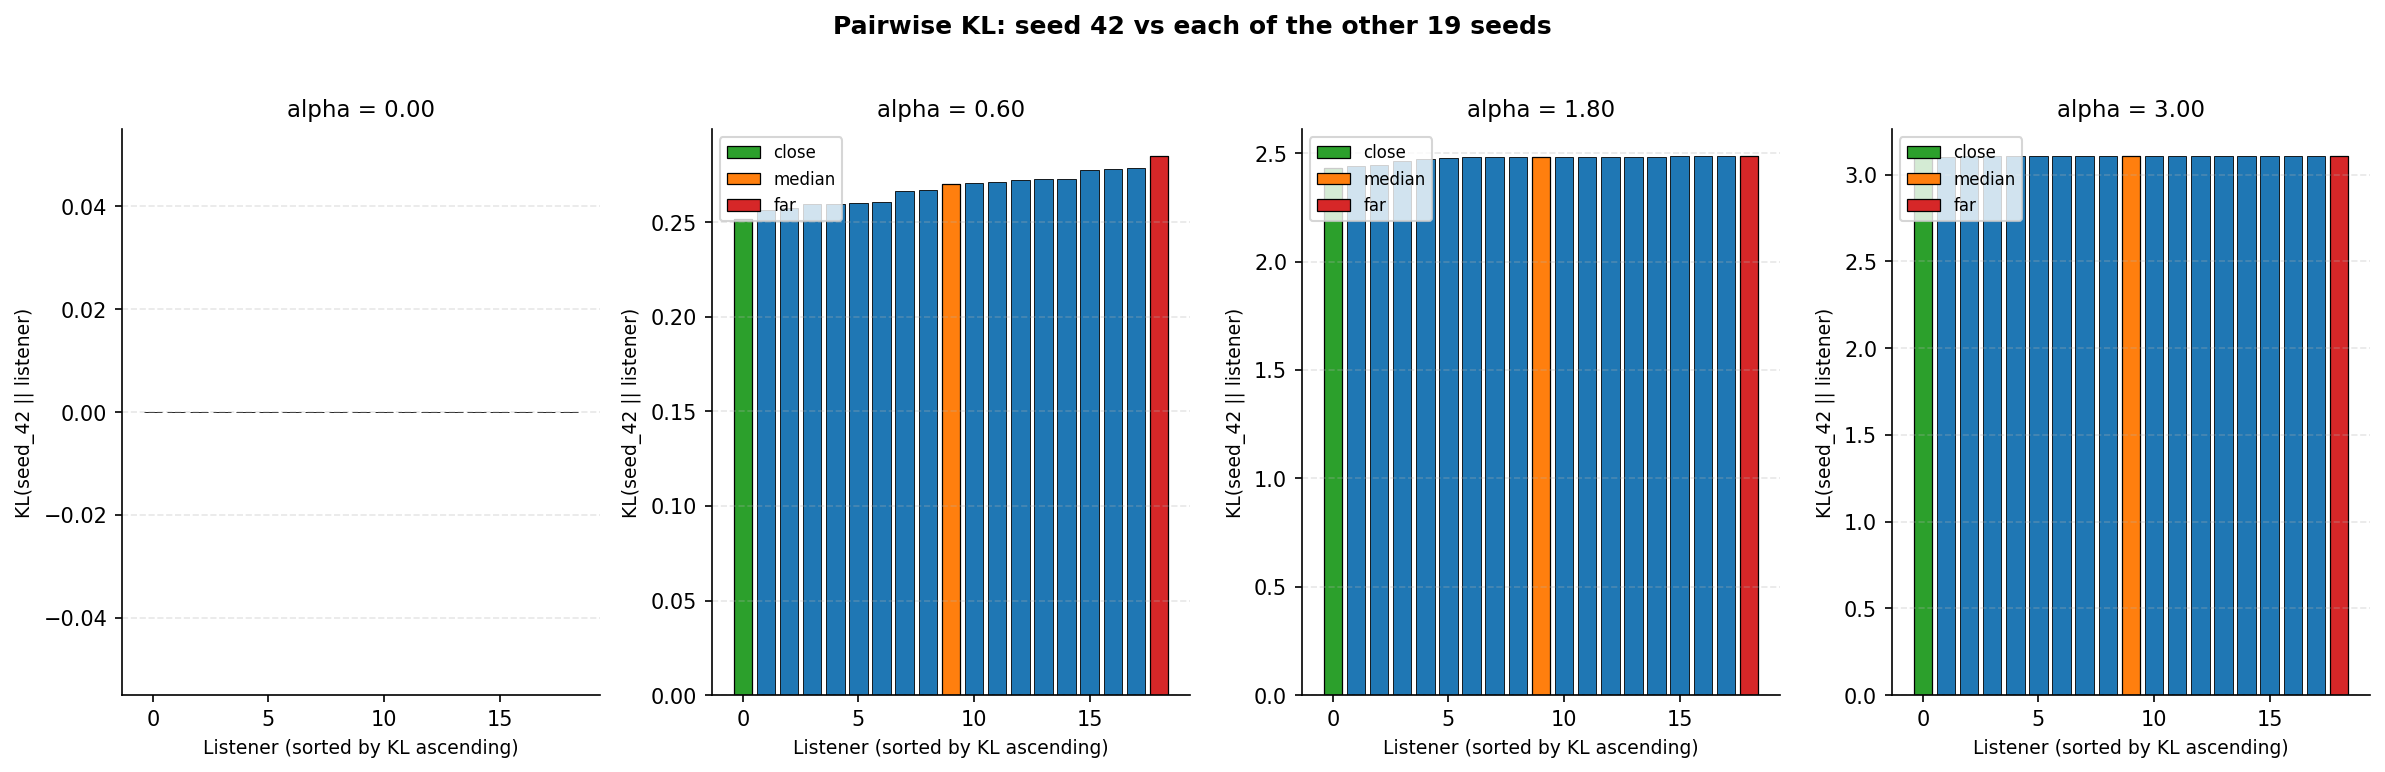
\includegraphics[width=0.95\textwidth]{images/kl_distribution_seed42.png}}{\missingfigure{images/kl_distribution_seed42.png}}
    \caption{Pairwise KL divergence between seed 42 and each of the other 19 seeds, on the pair-frequency distribution, at four representative $\alpha$ values ($0.00$, $0.60$, $1.80$, $3.00$).}
    \label{fig:rq3-pairwise-kl-distribution}
\end{figure}

\begin{figure}[htbp]
    \centering
    \IfFileExists{images/kl_subseq_distribution_seed42.png}{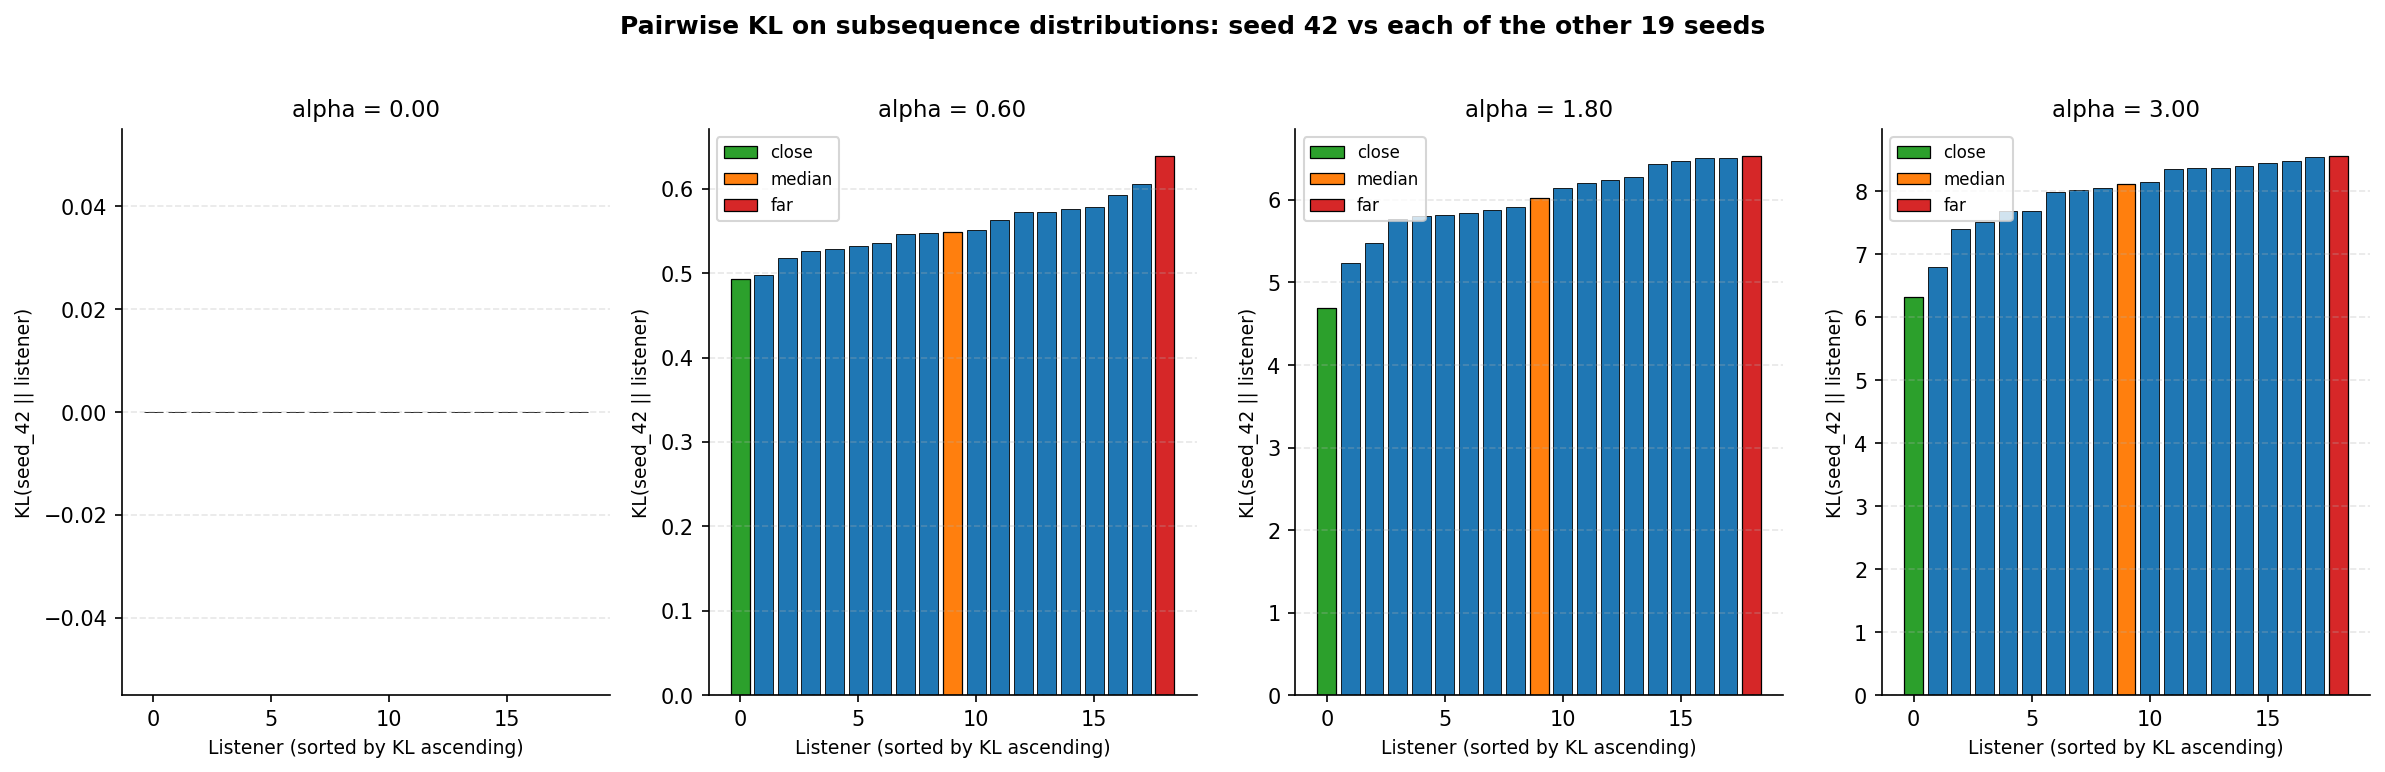
\includegraphics[width=0.95\textwidth]{images/kl_subseq_distribution_seed42.png}}{\missingfigure{images/kl_subseq_distribution_seed42.png}}
    \caption{Pairwise KL divergence between seed 42 and each of the other 19 seeds, on the subsequence distribution, at the same four $\alpha$ values.}
    \label{fig:rq3-subseq-kl-distribution}
\end{figure}

The pair-frequency KL is very compressed. At $\alpha = 3.00$, the 19 listeners span only 0.1\% of the mean distance from the speaker, making the close, median, and far positions statistically indistinguishable. This compression follows from the setup: all 20 seeds share the same Zipfian shape, and only the identity of the pair at each rank changes. With independent random permutations, the top pair of one seed lands roughly uniformly between rank 1 and rank 961 in another seed's ranking, so the KL is dominated by near-random alignment of the high-frequency mass. Under this metric, all 19 candidate listeners are approximately equally far from the speaker.

The subsequence-KL spreads the listeners by 26 to 31 percent across the three $\alpha$ values, which is much more informative. The Jaccard spreads them by 187 percent at $\alpha = 0.60$ and 158 percent at $\alpha = 1.80$, with a clean ordering from very high overlap (up to 0.83) down to zero overlap. At $\alpha = 3.00$ the Jaccard becomes degenerate, because all 19 candidate seeds share zero abstractions with seed 42, a consequence of the collapse regime we already documented in Chapter~\ref{ch:rq2}.

\subsection{Results Across the Three Metrics}
\label{sec:rq3-c-results}

Figures~\ref{fig:rq3-c-pair-kl},~\ref{fig:rq3-c-subseq-kl}, and~\ref{fig:rq3-c-jaccard} show the full accuracy curves. Table~\ref{tab:rq3-c-summary} summarises the quantities that matter for interpretation: the plateau reached by the cross-listeners, the approximate time needed to cross the 0.95 threshold, and whether the close/median/far ordering predicted by the distance metric appears.

\begin{figure}[htbp]
    \centering
    \IfFileExists{images/rq3_pair_kl_accuracy.png}{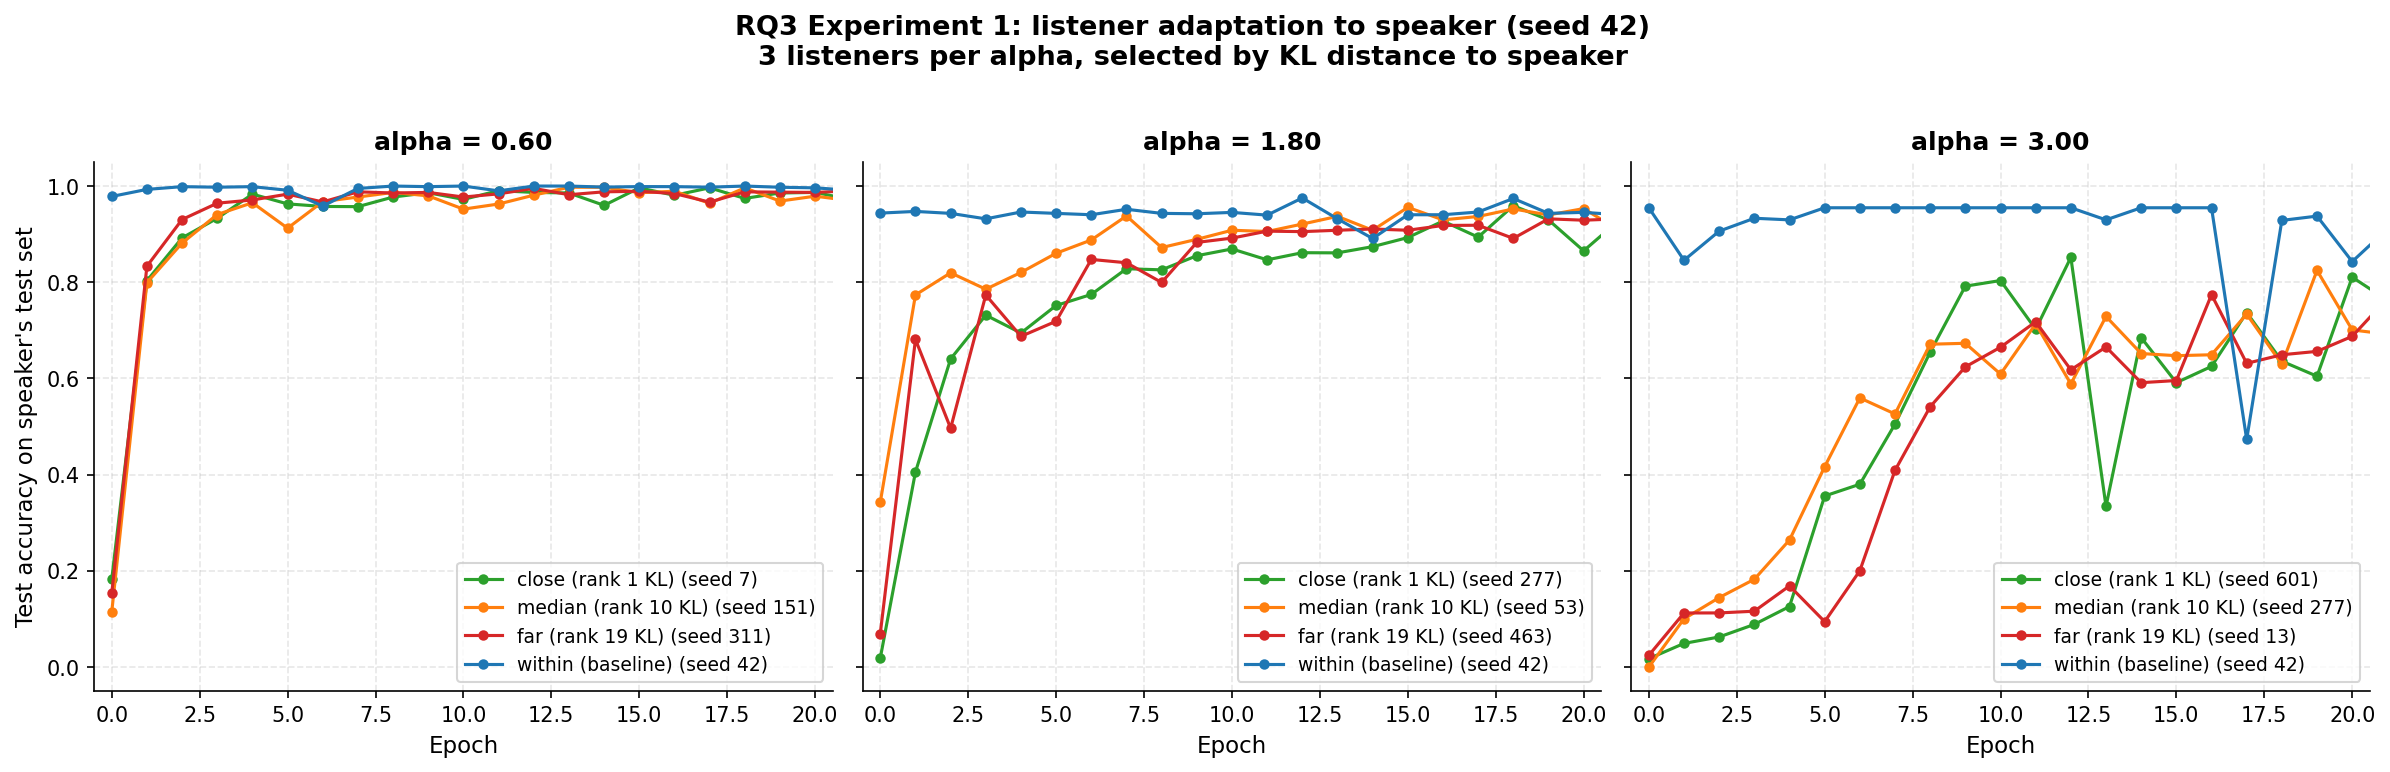
\includegraphics[width=1.0\textwidth]{images/rq3_pair_kl_accuracy.png}}{\missingfigure{images/rq3_pair_kl_accuracy.png}}
    \caption{Same-$\alpha$ cross-pairing under pair-frequency KL selection. Each panel corresponds to one $\alpha$, and each panel shows the within-baseline, close, median, and far listener curves over 20 epochs.}
    \label{fig:rq3-c-pair-kl}
\end{figure}

\begin{figure}[htbp]
    \centering
    \IfFileExists{images/rq3_subseq_kl_accuracy.png}{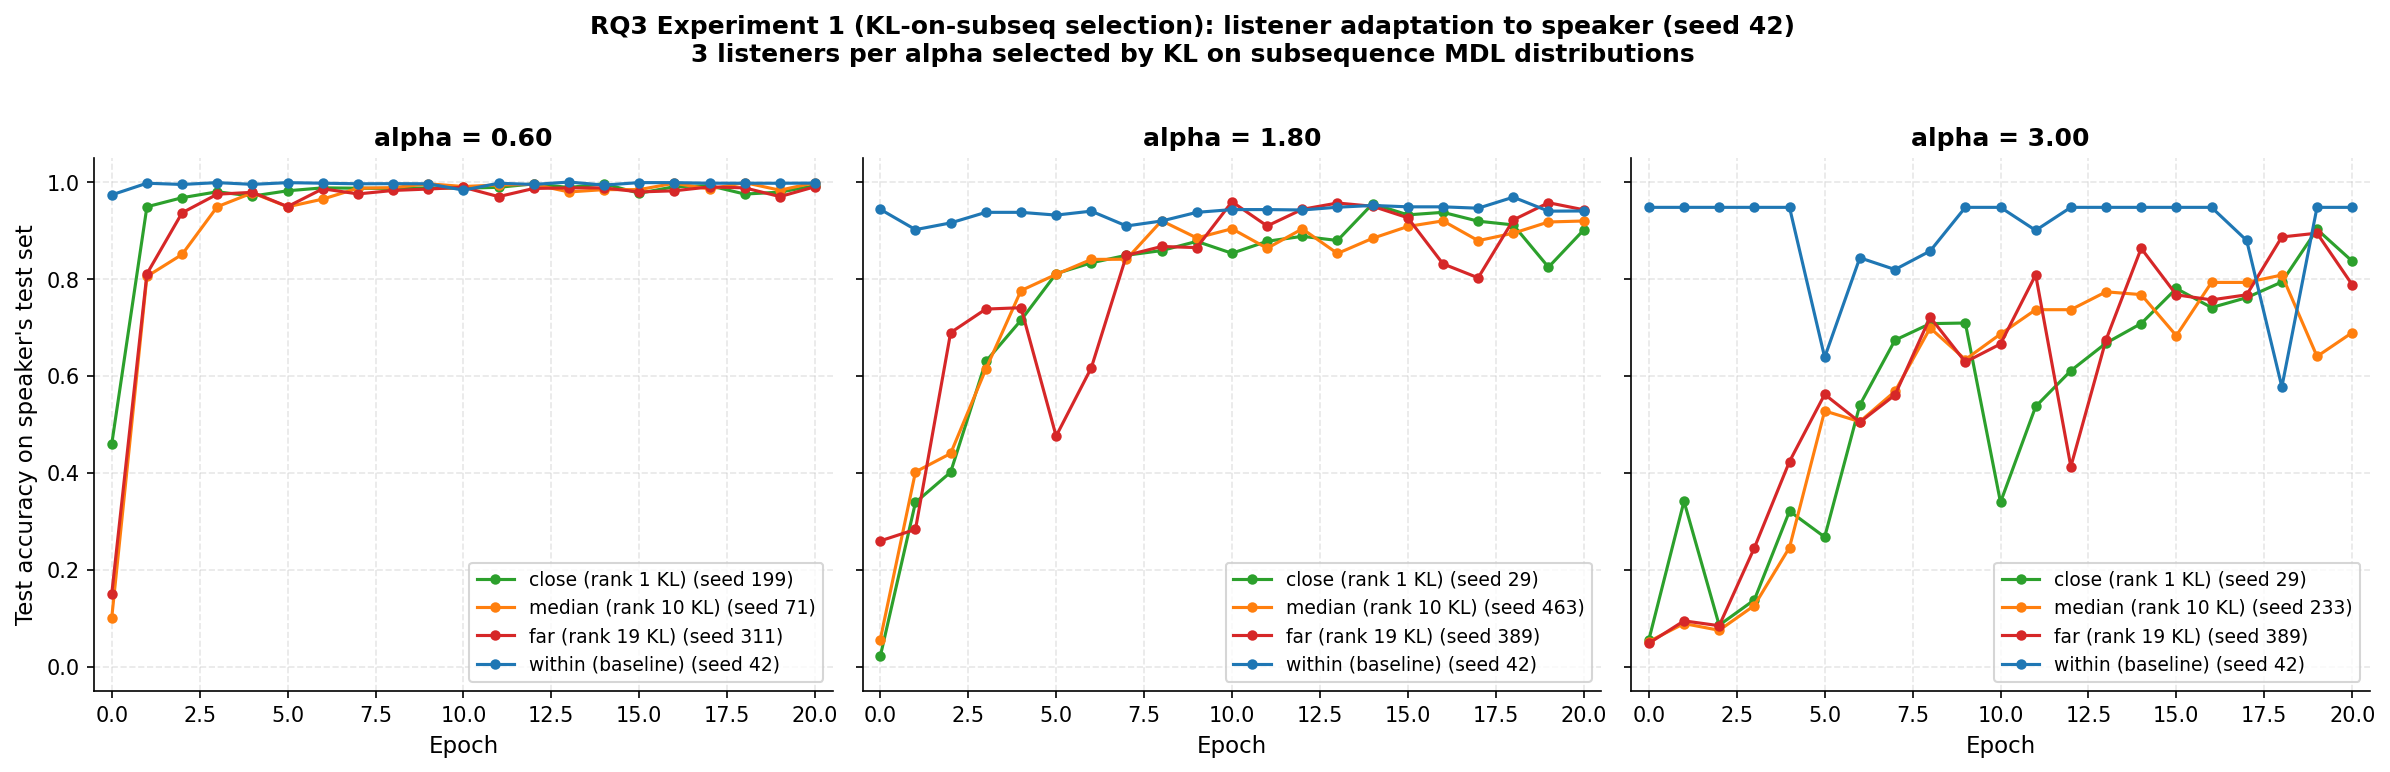
\includegraphics[width=1.0\textwidth]{images/rq3_subseq_kl_accuracy.png}}{\missingfigure{images/rq3_subseq_kl_accuracy.png}}
    \caption{Same-$\alpha$ cross-pairing under subsequence-KL listener selection.}
    \label{fig:rq3-c-subseq-kl}
\end{figure}

\begin{figure}[htbp]
    \centering
    \IfFileExists{images/rq3_jaccard_accuracy.png}{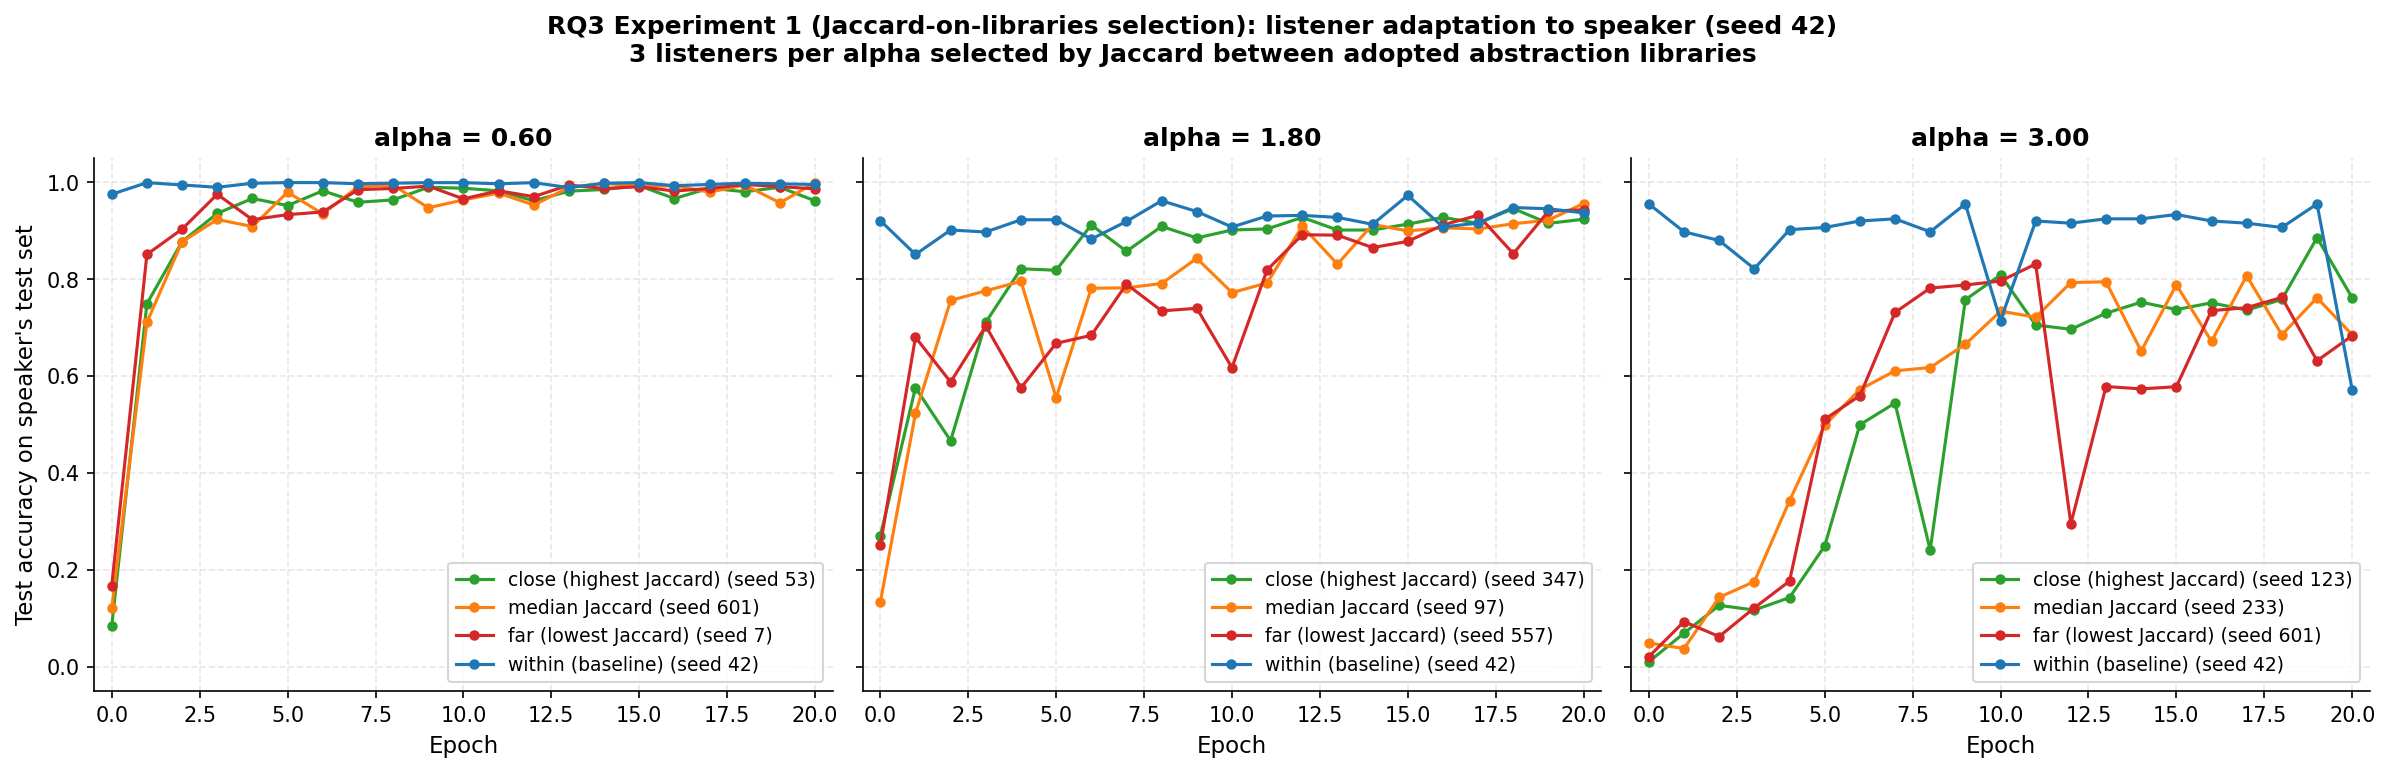
\includegraphics[width=1.0\textwidth]{images/rq3_jaccard_accuracy.png}}{\missingfigure{images/rq3_jaccard_accuracy.png}}
    \caption{Same-$\alpha$ cross-pairing under Jaccard listener selection.}
    \label{fig:rq3-c-jaccard}
\end{figure}

\begin{table}[htbp]
\small
\setlength{\tabcolsep}{4pt}
\begin{tabularx}{\textwidth}{ll>{\raggedright\arraybackslash}X>{\raggedright\arraybackslash}X>{\raggedright\arraybackslash}X}
\toprule
Selection metric & $\alpha$ & Plateau & Convergence & Distance ordering \\
\midrule
Pair-frequency KL & 0.60 & $\approx 0.98$ & threshold within 2 epochs & absent \\
Pair-frequency KL & 1.80 & $0.92$--$0.94$ & threshold in 6--13 epochs & absent \\
Pair-frequency KL & 3.00 & $\approx 0.71$ & threshold not reached & absent \\
Subsequence-KL & 0.60 & $\approx 0.99$ & fast & transient at epoch 0 only \\
Subsequence-KL & 1.80 & $\approx 0.90$ & slower & absent \\
Subsequence-KL & 3.00 & below threshold & -- & reversed/absent \\
Jaccard & 0.60 & $\approx 0.98$ & fast & absent \\
Jaccard & 1.80 & $0.867$--$0.916$ & -- & weak monotone ordering \\
Jaccard & 3.00 & $0.66$--$0.76$ & threshold not reached & degenerate \\
\bottomrule
\end{tabularx}
\caption{Summary of same-$\alpha$ cross-pairing outcomes. ``Threshold'' refers to reconstruction accuracy 0.95.}
\label{tab:rq3-c-summary}
\end{table}

The table makes the main result visible without relying on the identity of individual seeds. Adaptation difficulty is organised primarily by the shared concentration regime. Low concentration is easy, intermediate concentration is slower and remains below the within-pairing baseline, and high concentration fails to recover within the 20-epoch window. By contrast, the listener's position under the chosen distance metric rarely predicts the plateau. The only partial exception is Jaccard at $\alpha = 1.80$, where the close, median, and far listeners form a weak monotone ordering; even there, the gap is small and each position is represented by a single seed.

\subsection{What the Same-$\alpha$ Results Tell Us}
\label{sec:rq3-c-interpretation}

The three metrics agree on the essentials. Adaptation difficulty is governed mainly by the regime both agents inhabit: cross-listeners converge quickly at $\alpha = 0.60$, more slowly and below the within-baseline at $\alpha = 1.80$, and fail to cross the 0.95 threshold within 20 epochs at $\alpha = 3.00$. Within a fixed $\alpha$, speaker-listener distance is a weak predictor regardless of how distance is defined. Pair-frequency KL is too compressed to discriminate listeners, subsequence-KL does not produce a stable ordering, and Jaccard only shows a faint signal at $\alpha = 1.80$. That Jaccard is the only partial exception is suggestive, because it compares the vocabularies the agents actually built rather than the distributions they trained on. Still, the effect is small relative to the regime effect and is based on a single seed per position, so a cleaner test would need many more listeners per condition or a setup where the listener cannot rapidly retrain its neural mapping.

At $\alpha = 3.00$, even the within-baseline plateaus at only 0.933 rather than close to 1.0. When speaker and listener are literally the same trained agent, the plateau is still not perfect. This suggests that at high concentration the speaker's own communicative language is already somewhat degraded: even the speaker's own listener has non-trivial difficulty interpreting its messages. This is consistent with the collapse-regime findings of Chapter~\ref{ch:experimental}, where aggressive compression at high $\alpha$ produced short but idiosyncratic programs that are harder to interpret even for the agent that produced them.

\section{Adaptation Dynamics Under Modifications to the Base Setup (Group M)}
\label{sec:rq3-group-m}

\subsection{Why We Introduced Modifications}
\label{sec:rq3-m-motivation}

The results of Section~\ref{sec:rq3-group-c} give us a clear outcome (adaptation is regime-dependent), but they leave the mechanism behind that outcome opaque. What is the bandit doing during joint training that makes low-$\alpha$ cases easy and high-$\alpha$ cases hard? The base setup measures the outcome (accuracy) but does not expose the underlying trajectory of the bandit's decisions or the neural adaptation of the listener. To open up that black box, we introduced three modifications to the base setup, each targeting a different aspect and each producing a different lens on the dynamics.

Modification M1, which we call revert-to-primitives, enlarges the bandit's action space at joint-training time. In the base setup the bandit chooses among trajectories that all use the speaker's adopted abstractions. In M1 we also give the bandit the option to select a primitive-only trajectory for each scene. This lets us watch whether the bandit consolidates on the speaker's abstractions or falls back to primitives when the listener has trouble interpreting them.

Modification M2, pretraining on primitives, adds one epoch of supervised pretraining of the listener on the shared primitive vocabulary before joint training begins. The aim is to separate two things that happen in parallel during adaptation: the neural phase, in which the listener re-aligns its decoder on the speaker's 2 primitive tokens, and the symbolic phase, in which the bandit decides which abstractions to keep or drop. By accelerating the neural phase with pretraining, we can see whether the symbolic phase is qualitatively different from what we observed without pretraining.

Modification M3, increased bandit exploration, raises the bandit's $\varepsilon$ from 0.1 (the PACE default) to 0.2 and 0.4. This tests whether more exploration keeps the bandit from settling too early on primitives before the listener has had a chance to demonstrate its ability to interpret the abstractions.

We apply all three modifications at $\alpha = 1.80$, which is the case where Section~\ref{sec:rq3-group-c} shows a measurable but non-trivial adaptation and where the dynamics are therefore most informative to inspect.


\begin{table}[htbp]
\centering
\small
\setlength{\tabcolsep}{4pt}
\begin{tabularx}{\textwidth}{>{\raggedright\arraybackslash}p{0.22\textwidth}>{\raggedright\arraybackslash}X>{\raggedright\arraybackslash}X}
\toprule
Modification & Main diagnostic & Interpretation \\
\midrule
M1: revert to primitives & U-shaped abstraction Q-values & unlearn-then-relearn symbolic dynamic \\
M2: primitive pretraining & higher epoch-0 accuracy & neural alignment accelerates, symbolic dynamics remain \\
M3: higher $\varepsilon$ & higher retained abstraction Q-values & exploration protects abstractions from early abandonment \\
\bottomrule
\end{tabularx}
\caption{Summary of the three Group M modifications. The detailed curves are shown in Figures~\ref{fig:rq3-m1-dynamics},~\ref{fig:rq3-m2-dynamics}, and~\ref{fig:rq3-m3-dynamics}.}
\label{tab:rq3-m-summary}
\end{table}

\subsection{M1: Revert-to-Primitives}
\label{sec:rq3-m1}

\begin{figure}[htbp]
    \centering
    \IfFileExists{images/rq3_m1_dynamics.png}{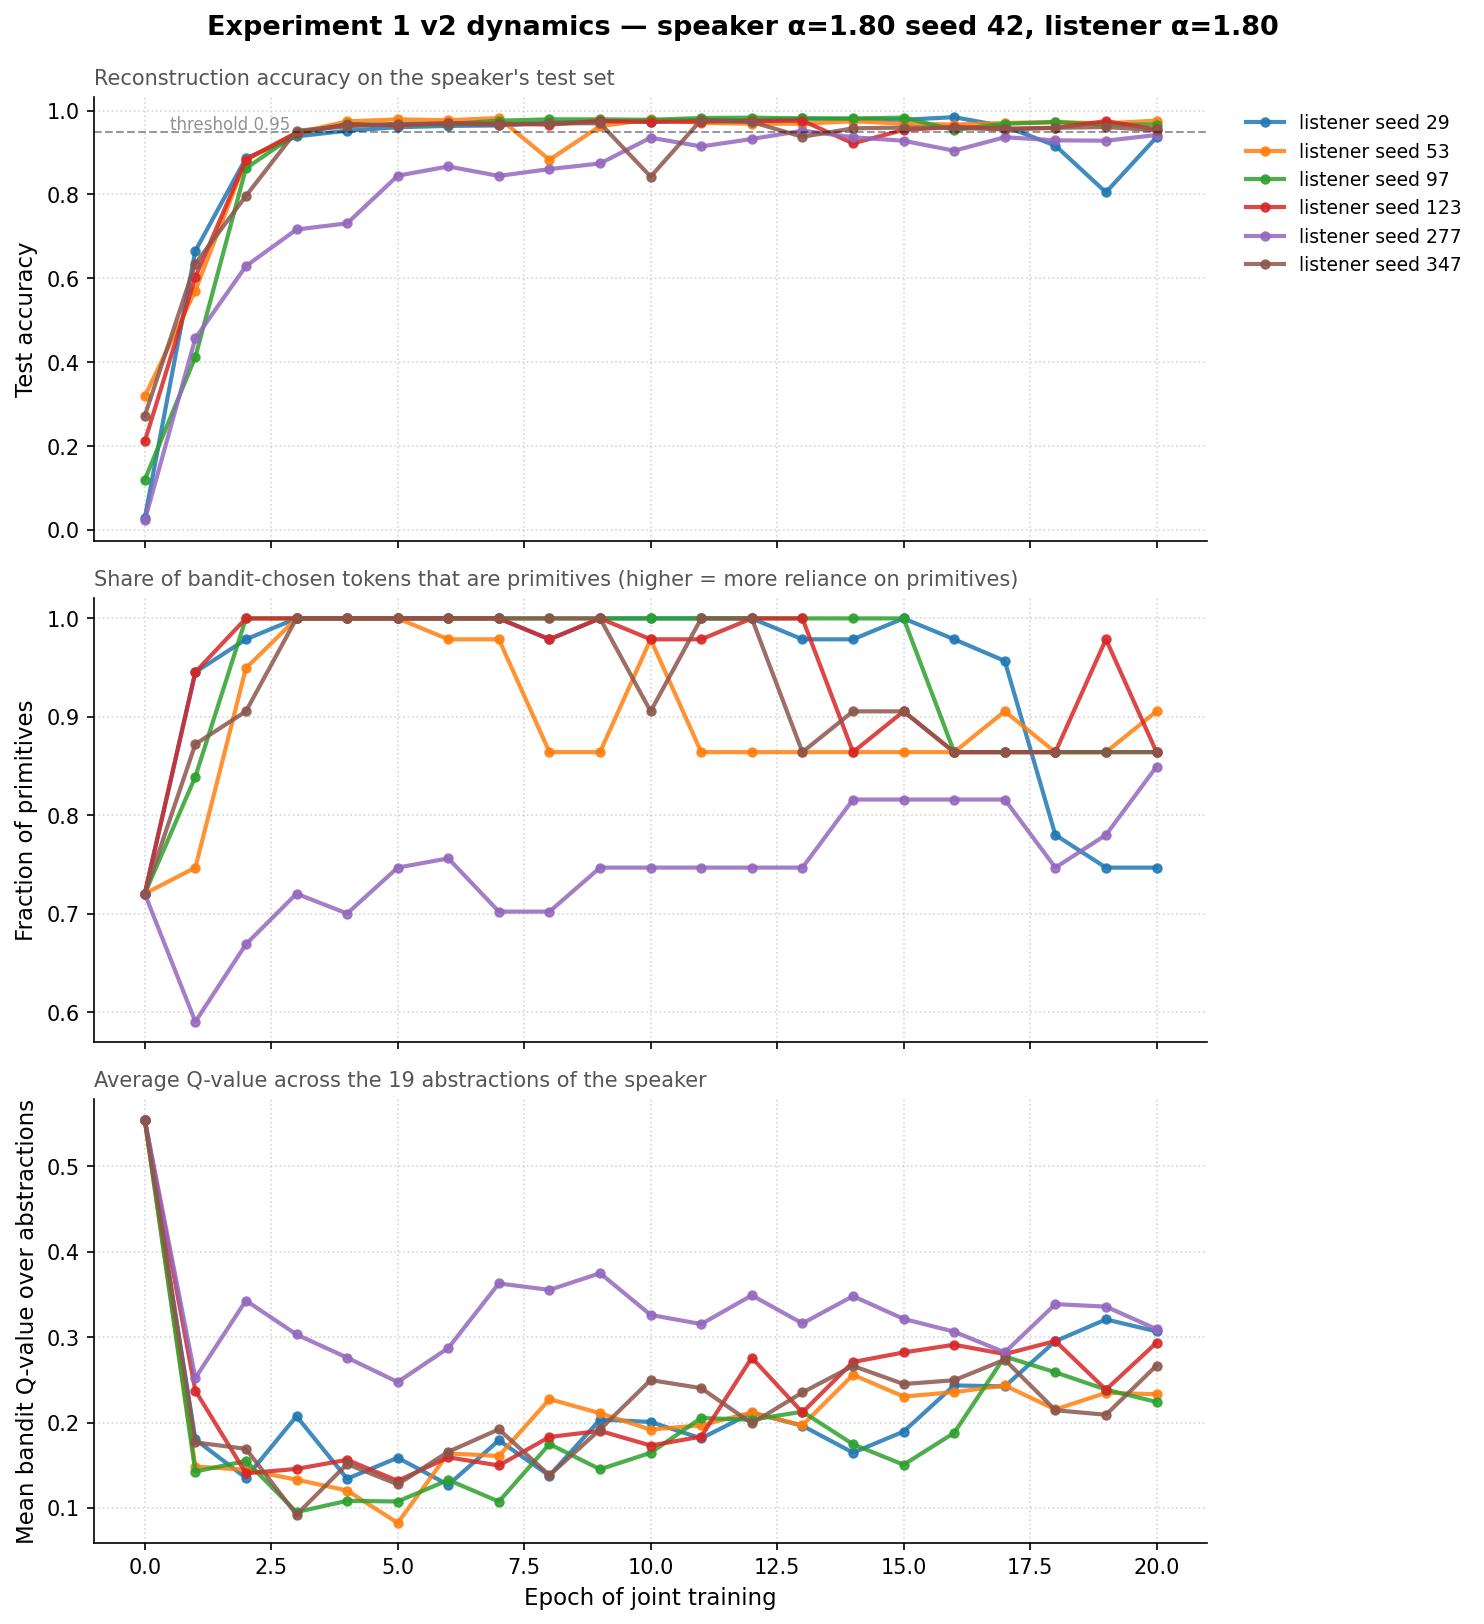
\includegraphics[width=0.95\textwidth]{images/rq3_m1_dynamics.png}}{\missingfigure{images/rq3_m1_dynamics.png}}
    \caption{M1 revert-to-primitives dynamics at $\alpha = 1.80$: test accuracy, fraction of primitives selected by the bandit, and mean Q-value over abstractions.}
    \label{fig:rq3-m1-dynamics}
\end{figure}

We pair the speaker ($\alpha = 1.80$, seed 42) with six listener seeds under M1. The useful signal is the common shape of the response rather than the exact trajectory of each seed. All listeners eventually reach the 0.95 threshold, but the bandit initially retreats from the speaker's abstractions and later partially returns to them. In the primitive-fraction panel this appears as an early shift toward primitive-only trajectories; in the Q-value panel it appears as a U-shaped curve over the speaker's abstractions. The initial drop is an unlearning phase, where the bandit receives evidence that the listener cannot yet interpret the abstractions. The later recovery begins once the listener's decoder has aligned enough for abstraction-using trajectories to become valuable again. M1 exposes this symbolic dynamic because it gives the bandit a genuine alternative to the speaker's abstractions; the base setup hides it because abstraction-using trajectories are the only available branch.

\subsection{M2: Pretraining on Primitives}
\label{sec:rq3-m2}

\begin{figure}[htbp]
    \centering
    \IfFileExists{images/rq3_m2_dynamics.png}{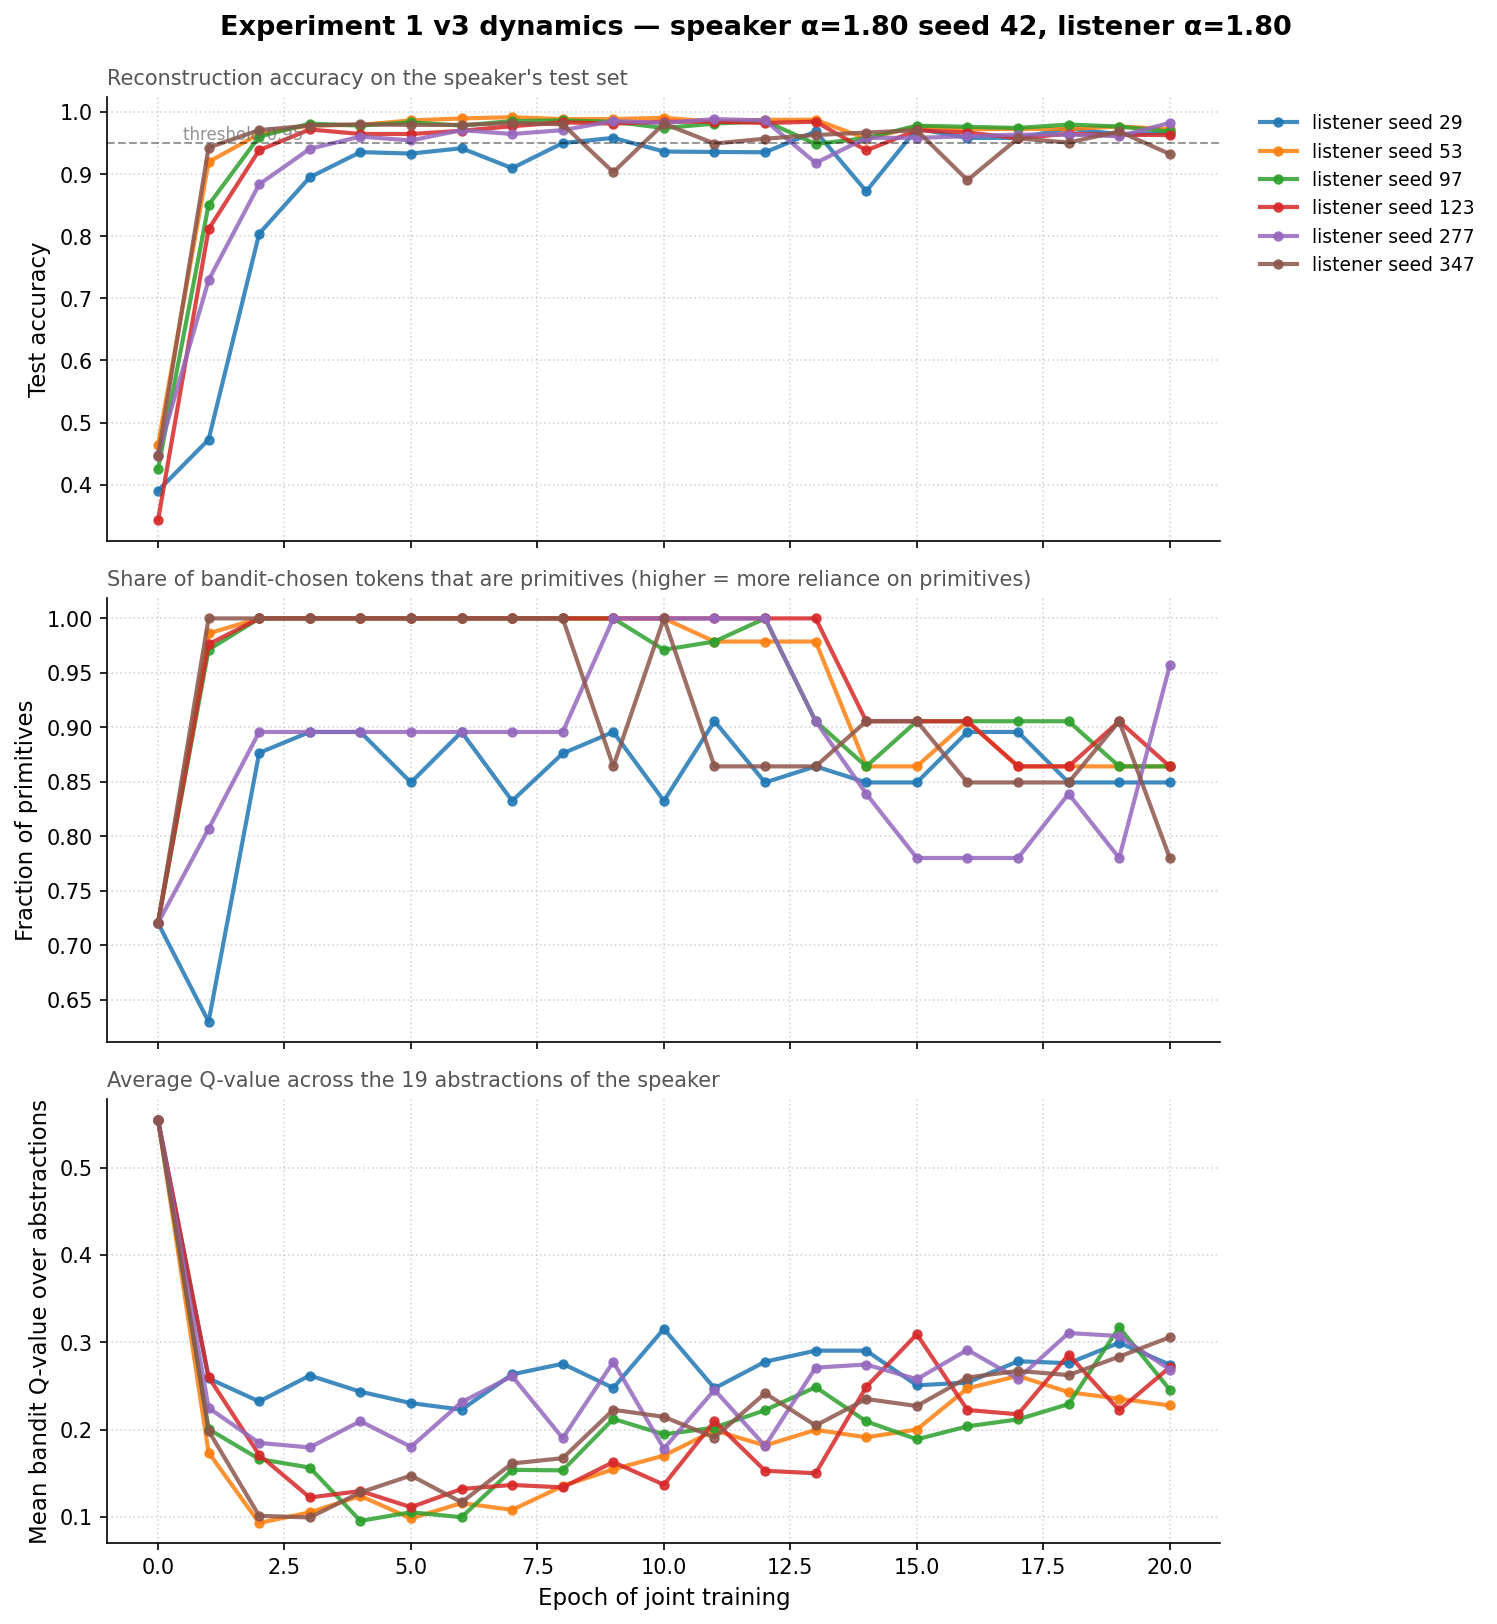
\includegraphics[width=0.95\textwidth]{images/rq3_m2_dynamics.png}}{\missingfigure{images/rq3_m2_dynamics.png}}
    \caption{M2 primitive-pretraining dynamics compared with M1. Solid lines show no pretraining and dashed lines show pretraining.}
    \label{fig:rq3-m2-dynamics}
\end{figure}

Pretraining raises epoch-0 accuracy for every listener, so it clearly accelerates the neural part of adaptation: the listener begins the interaction already better aligned on the shared primitive vocabulary. The symbolic phase remains, however. The primitive-fraction and mean-Q trajectories stay qualitatively similar to M1, with seed-level differences in speed but no change in the underlying pattern. The interpretation is therefore narrow: primitive pretraining helps the listener decode the basic tokens sooner, while the bandit still has to learn which speaker abstractions to trust, a question closely related to the learnability of semantic or symbolic systems~\cite{steinert-threlkeld_ease_2020}.

\subsection{M3: Increased Bandit Exploration}
\label{sec:rq3-m3}

\begin{figure}[htbp]
    \centering
    \IfFileExists{images/rq3_m3_dynamics.png}{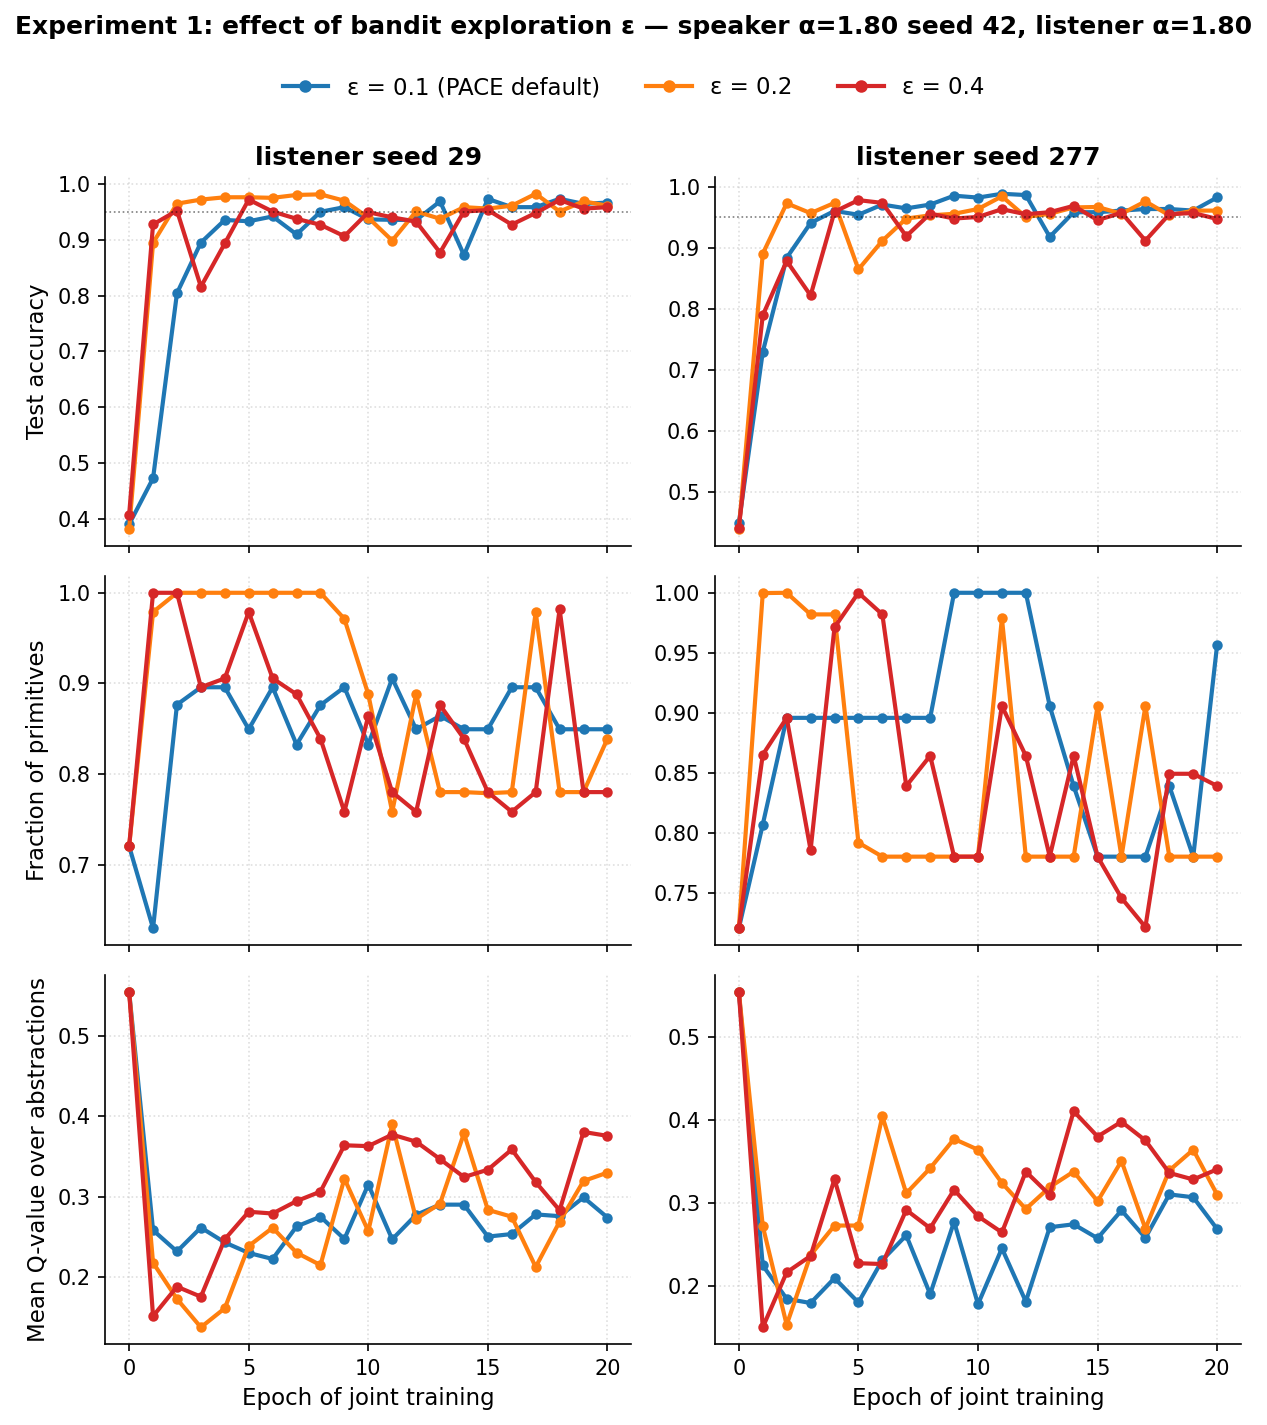
\includegraphics[width=0.95\textwidth]{images/rq3_m3_dynamics.png}}{\missingfigure{images/rq3_m3_dynamics.png}}
    \caption{M3 increased-exploration sweep at $\alpha = 1.80$, comparing $\varepsilon = 0.1$, $\varepsilon = 0.2$, and $\varepsilon = 0.4$ for listener seeds 29 and 277.}
    \label{fig:rq3-m3-dynamics}
\end{figure}

M3 tests whether the depth of the Q-value collapse depends on exploration. Across the two diagnostic listener seeds, higher $\varepsilon$ consistently preserves more mean Q-value in the speaker's abstractions, while test accuracy changes little. The primitive-fraction curves are noisier, especially at the highest exploration setting, but the direction of the Q-value result is clear: exploration gives abstractions more chances to prove useful before the bandit abandons them. This supports the reading of M1 as a symbolic trust dynamic rather than a purely neural failure.

\subsection{What the Three Modifications Tell Us Together}
\label{sec:rq3-m-summary}

Together the three modifications separate the neural and symbolic sides of adaptation. Giving the bandit a way to bypass the speaker's abstractions (M1) exposes an unlearn-then-relearn dynamic: Q-values drop sharply at first, then recover as the listener catches up. Pretraining the listener on primitives (M2) speeds up the neural side while leaving that symbolic trajectory largely unchanged, evidence that the two phases respond to different signals. Raising the exploration parameter (M3) preserves more Q-value in the abstractions by giving them more chances to prove useful before the bandit gives up on them. The same-$\alpha$ cross-pairing task therefore tests whether the listener can interpret the speaker's discrete vocabulary, and the bandit's response reveals how neural alignment and symbolic trust interact.

\section{Cross-$\alpha$ Pairing (Group X)}
\label{sec:rq3-group-x}

\subsection{Why go to Cross-$\alpha$}
\label{sec:rq3-x-motivation}

The same-$\alpha$ cross-pairing results of Section~\ref{sec:rq3-group-c} tell us that adaptation difficulty depends strongly on $\alpha$ but weakly on distance within a given $\alpha$. The natural next question is what happens when we pair agents that come from substantially different $\alpha$ values, so that the distance is much larger, not just in the ranking of frequent pairs but in the overall shape of the training distribution.

We consider two variants of this setup. In the frozen-speaker variant (X1), the speaker's weights and bandit state stay frozen for the entire joint training, and only the listener adapts. In the unfrozen-speaker variant (X2), both agents remain trainable and the optimiser updates both sets of neural weights. Comparing the two variants isolates the neural component of any cross-$\alpha$ gap. If the gap shrinks in the unfrozen setting, it must reflect at least partly a neural mismatch that a co-adapting speaker can help resolve. If the gap stays the same, it must be structural, a property of the two agents' training conditions that neural adaptation cannot address.

We run the full 21 by 21 grid of pairings for two speaker seeds (42 and 123). Two seeds are not a substitute for the twenty-seed variability we would want for a proper statistical claim, but they let us check whether the pattern we see on seed 42 also shows up on a different reference agent. We treat $n = 2$ as a robustness check, not as a population estimate.

\subsection{X1: Frozen Speaker}
\label{sec:rq3-x1}

\begin{figure}[htbp]
    \centering
    \IfFileExists{images/rq3_x1_curves.png}{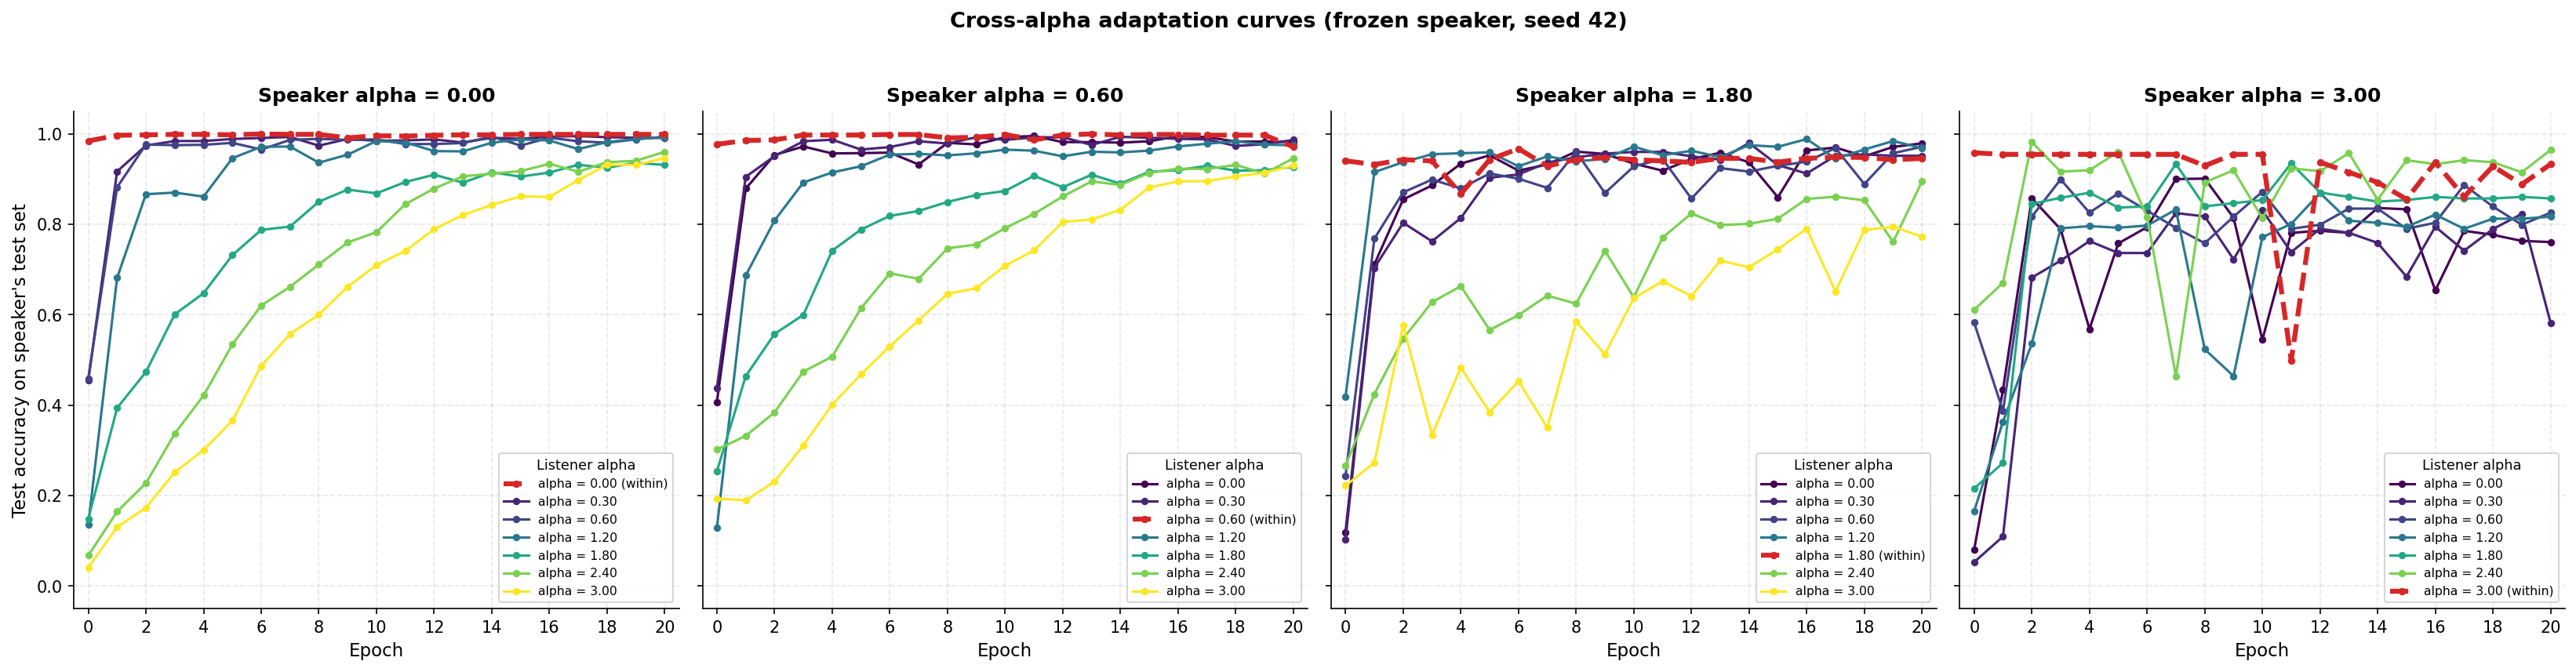
\includegraphics[width=0.95\textwidth]{images/rq3_x1_curves.png}}{\missingfigure{images/rq3_x1_curves.png}}
    \caption{Frozen-speaker cross-$\alpha$ adaptation curves for seed 42.}
    \label{fig:rq3-x1-curves}
\end{figure}

\begin{figure}[htbp]
    \centering
    \IfFileExists{images/rq3_x1_summary.png}{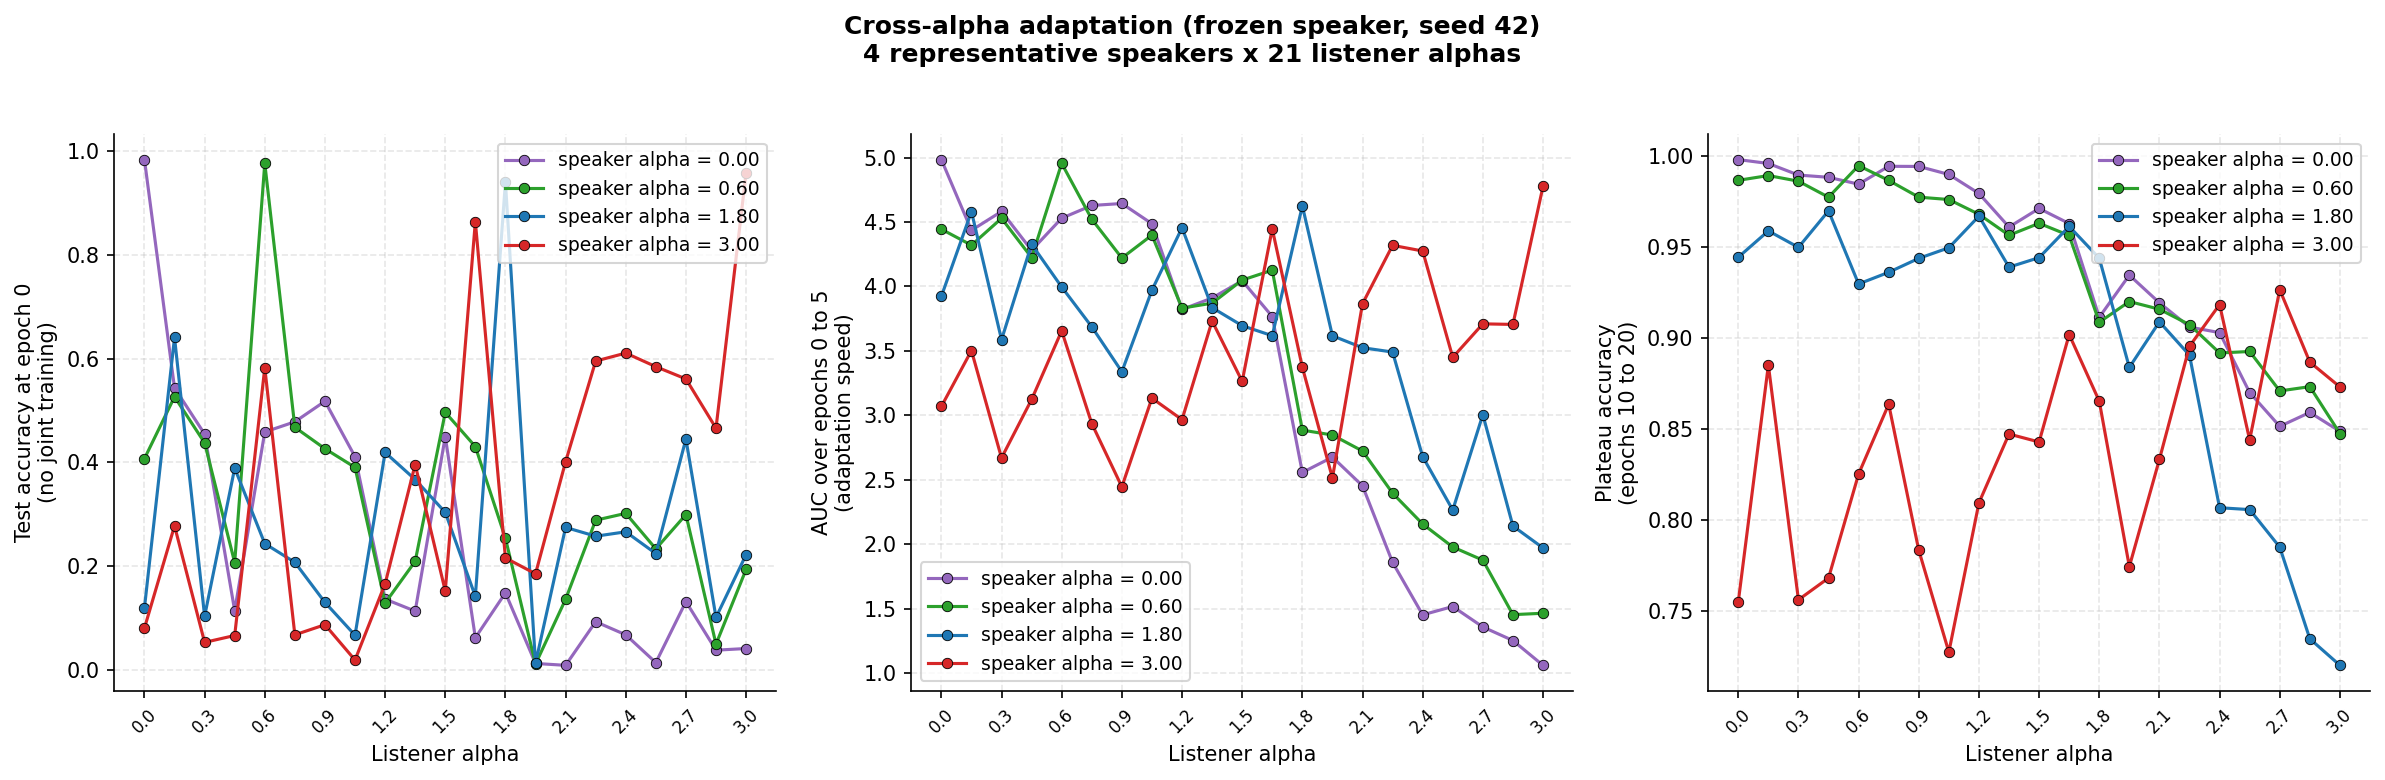
\includegraphics[width=0.95\textwidth]{images/rq3_x1_summary.png}}{\missingfigure{images/rq3_x1_summary.png}}
    \caption{Frozen-speaker cross-$\alpha$ summary metrics for seed 42.}
    \label{fig:rq3-x1-summary}
\end{figure}

The frozen-speaker sweep is dominated by the speaker's training regime. Speakers trained at $\alpha = 0.00$ or $\alpha = 0.60$ pair robustly with listeners from the whole range, with plateaus above 0.95 for most listeners and only a gradual decline as listener concentration increases. Speakers trained at $\alpha = 1.80$ settle lower, around 0.90 to 0.94. Speakers trained at $\alpha = 3.00$ are the hardest to interpret, with plateaus in the 0.75 to 0.90 range and much larger variability. The asymmetry is visible in direct comparisons: (sp = 3.00, li = 0.60) plateaus at 0.83, while (sp = 0.60, li = 3.00) reaches 0.93.

The mechanism we propose for this asymmetry is the following. A concentrated speaker has a small library of abstractions that are highly specialised to the few pairs that are frequent in its dataset. When paired with a listener from a different regime, the listener has to interpret abstractions that reflect a very specific and narrow set of scenes, and there is little shared structural ground to work with. A uniform speaker has a broader library that generalises across many scenes, and any listener has a higher chance of encountering enough shared structural motifs to bootstrap the adaptation. This reading is consistent with the collapse-regime findings of Chapters~\ref{ch:experimental} and~\ref{ch:rq2}, where high-$\alpha$ agents were shown to produce short and idiosyncratic programs.

The listener's regime still modulates adaptability. For a fixed uniform speaker, moving the listener from $\alpha = 0.00$ to $\alpha = 3.00$ lowers the plateau by about 15 percent. The effect is real, but it remains secondary to the speaker-side effect.

\subsection{X2: Unfrozen Speaker}
\label{sec:rq3-x2}

\begin{figure}[htbp]
    \centering
    \IfFileExists{images/rq3_x2_curves.png}{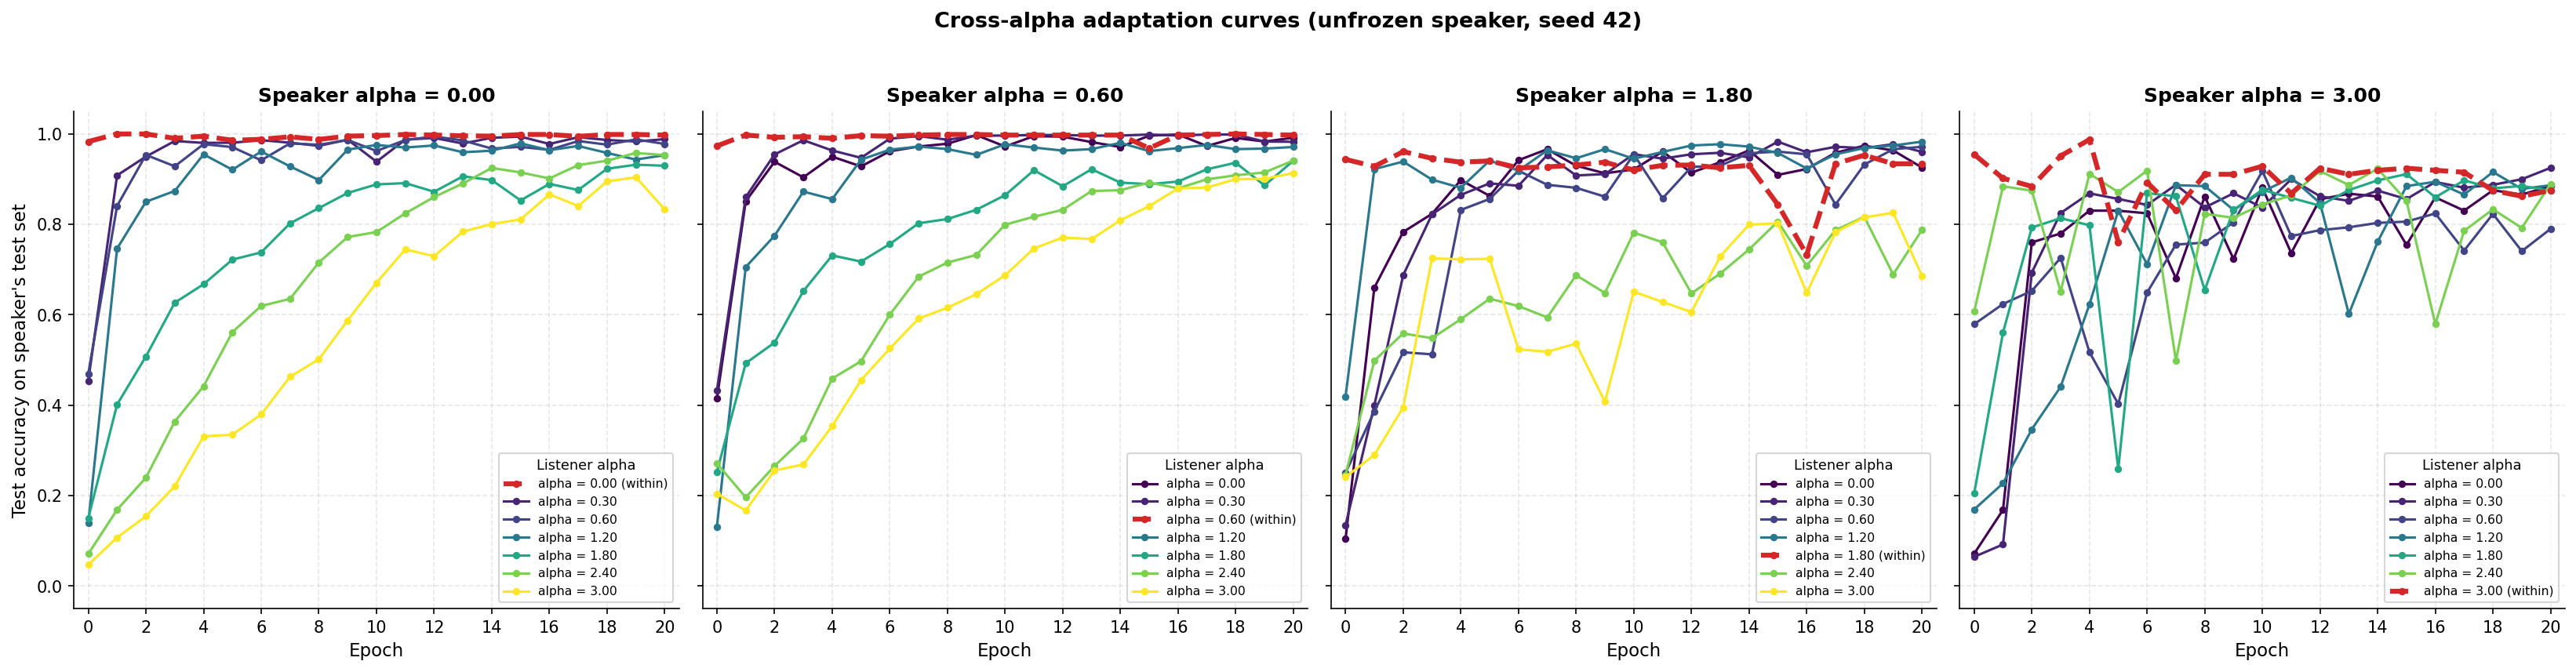
\includegraphics[width=0.95\textwidth]{images/rq3_x2_curves.png}}{\missingfigure{images/rq3_x2_curves.png}}
    \caption{Unfrozen-speaker cross-$\alpha$ adaptation curves for seed 42.}
    \label{fig:rq3-x2-curves}
\end{figure}

\begin{figure}[htbp]
    \centering
    \IfFileExists{images/rq3_x2_summary.png}{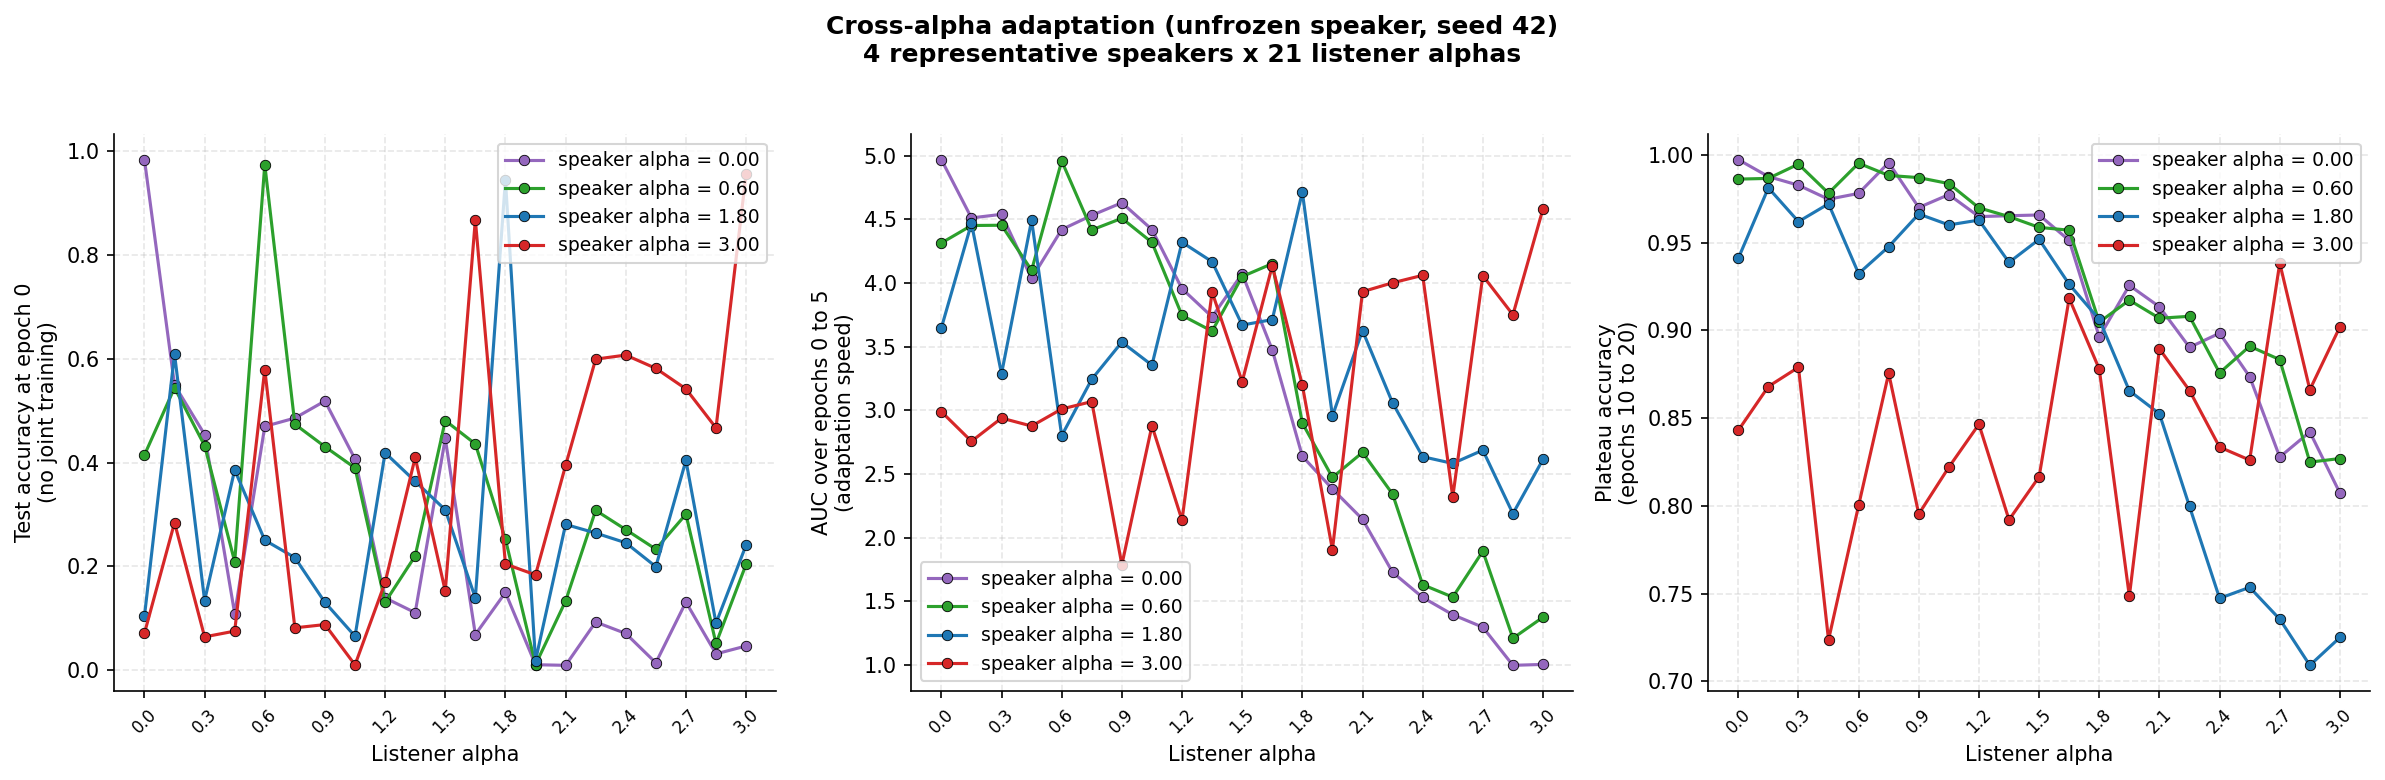
\includegraphics[width=0.95\textwidth]{images/rq3_x2_summary.png}}{\missingfigure{images/rq3_x2_summary.png}}
    \caption{Unfrozen-speaker cross-$\alpha$ summary metrics for seed 42.}
    \label{fig:rq3-x2-summary}
\end{figure}

The unfrozen-speaker sweep produces plateau values that are qualitatively very similar to the frozen-speaker sweep. Speakers at $\alpha = 0.00$ and 0.60 pair well with any listener; speakers at $\alpha = 3.00$ do not. The magnitude of the gap is essentially the same as in the frozen case. One small difference: the within-baseline plateaus become slightly less stable in the unfrozen setting, presumably because the speaker's own weights are drifting during joint training and the listener is trying to hit a moving target.

The bottom line is that letting the speaker adapt neurally during joint training leaves the cross-$\alpha$ gap in place. The bottleneck lies in the coverage and specificity of the vocabularies built during training. Neural adaptation can be one-sided or two-sided, but it cannot compensate for a mismatch at the level of the discrete vocabulary.

\subsection{What Cross-$\alpha$ Tells Us That Same-$\alpha$ Cannot}
\label{sec:rq3-x-interpretation}

Cross-$\alpha$ pairing exposes a structural bottleneck that same-$\alpha$ pairing cannot detect, because same-$\alpha$ pairing keeps the two agents in the same distributional regime. Same-$\alpha$ difficulty (Section~\ref{sec:rq3-group-c}) is regime-driven and roughly symmetric: it depends on the $\alpha$ that both agents share. Cross-$\alpha$ difficulty (Section~\ref{sec:rq3-group-x}) is asymmetric and driven by vocabulary coverage: it depends primarily on the speaker's $\alpha$, with the listener's $\alpha$ playing a secondary modulating role.

The comparison between frozen and unfrozen speakers also clarifies the role of the modifications in Section~\ref{sec:rq3-group-m}. M1, M2, and M3 operate on the neural or exploration side of the setup, so they can reshape local adaptation dynamics without addressing the structural gap. When two libraries are too specialised or too poorly overlapping to support communication, local tuning during joint training is insufficient.

\section{Case Studies Beyond Training Distribution (Group O)}
\label{sec:rq3-group-o}

\subsection{Why Case Studies and Not Sweeps}
\label{sec:rq3-o-framing}

The remaining two setups are treated as case studies rather than as full sweeps. The reason is that the cross-$\alpha$ results of Section~\ref{sec:rq3-group-x} already give a systematic test of training-distribution mismatch, and further sweeps would not add much to that picture. The case studies here probe two qualitatively different setups. The first is what happens when two agents interact on a dataset that is a mixture of both of their training distributions (O1). The second is what happens when a single agent is exposed to a distributional environment it never encountered during training (O2, with a qualitative follow-up in O3).

\subsection{O1: Mixed-Distribution Interaction}
\label{sec:rq3-o1}

\begin{figure}[htbp]
    \centering
    \IfFileExists{images/rq3_o1_mixed.png}{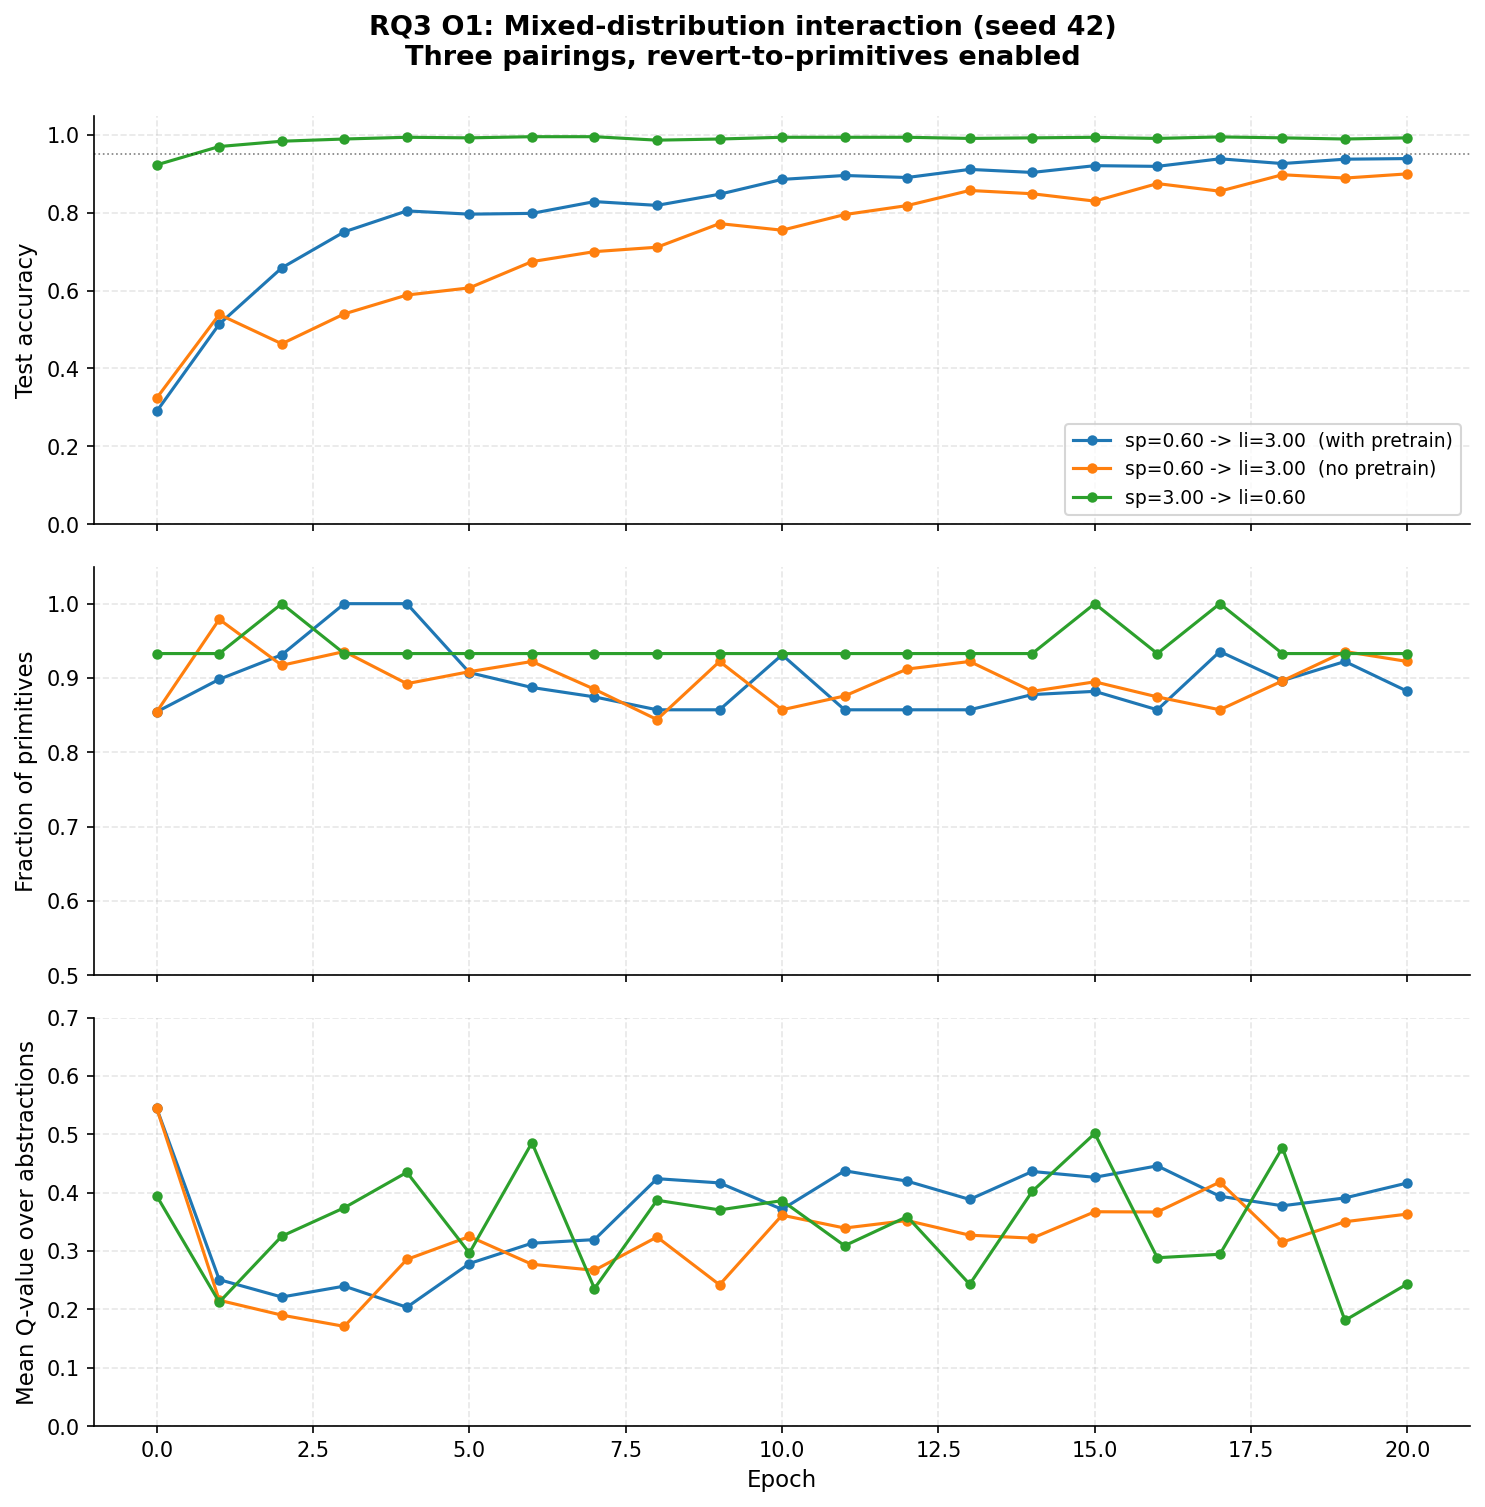
\includegraphics[width=0.85\textwidth]{images/rq3_o1_mixed.png}}{\missingfigure{images/rq3_o1_mixed.png}}
    \caption{Mixed-distribution interaction dynamics.}
    \label{fig:rq3-o1-mixed}
\end{figure}

The mixed-distribution setup pairs a speaker at one $\alpha$ with a listener at another $\alpha$ on a 50/50 mixture of their two training datasets, with the revert-to-primitives option enabled at joint-training time. The idea was that shared exposure to both distributions might produce an unlearning dynamic, in which the bandit drops abstractions that work well for one distribution but not for the other.

The three pairings we ran tell a consistent story. In the pairing (sp = 0.60, li = 3.00) with pretraining, accuracy climbs from 0.29 to 0.94 over 20 epochs, but the fraction of primitives stays around 0.88 throughout and the mean Q-value drops modestly from 0.55 to 0.42. Without pretraining, the same pairing has a similar but slower trajectory: accuracy from 0.32 to 0.90, fraction of primitives ending at 0.92, mean Q-value ending at 0.36. In the pairing (sp = 3.00, li = 0.60), accuracy is already at 0.92 at epoch 0 and reaches 0.99 by epoch 5, while the fraction of primitives and the mean Q-value are essentially flat throughout.

The setup does not produce a substantial unlearning dynamic in any of the three pairings. The fraction of primitives moves by less than 8 percent in every case, and the mean Q-value declines only modestly. The reason is structural, and it is the same one we already saw at work in the fast collapse of M1. A primitive-only trajectory has a Q-value close to 1.0 across all tokens, because the reward for primitives is deterministic. An abstraction-using trajectory has at least one lower-Q token that drags the mean down. Unless the listener already interprets the abstractions well from the very start, the primitive branch wins the bandit's selection by construction, and no unlearning dynamic can emerge.

This is a negative result, but an informative one. It tells us that the revert-to-primitives modification, which we designed to expose unlearning at the level of individual abstractions, carries a structural bias toward primitives whenever the listener does not initially understand the abstractions. The same mechanism produces the fast collapse of the fraction of primitives to 1.0 in five of the six seeds of M1, and the shallow flat trajectory in the mixed-distribution setup here. In both cases, the primitive branch dominates because it is deterministically reliable, and the abstractions have no way to compete unless the listener demonstrates its interpretation of them from the start.

\subsection{O2: Out-of-Distribution Shift}
\label{sec:rq3-o2}

\begin{figure}[htbp]
    \centering
    \IfFileExists{images/rq3_o2_overview.png}{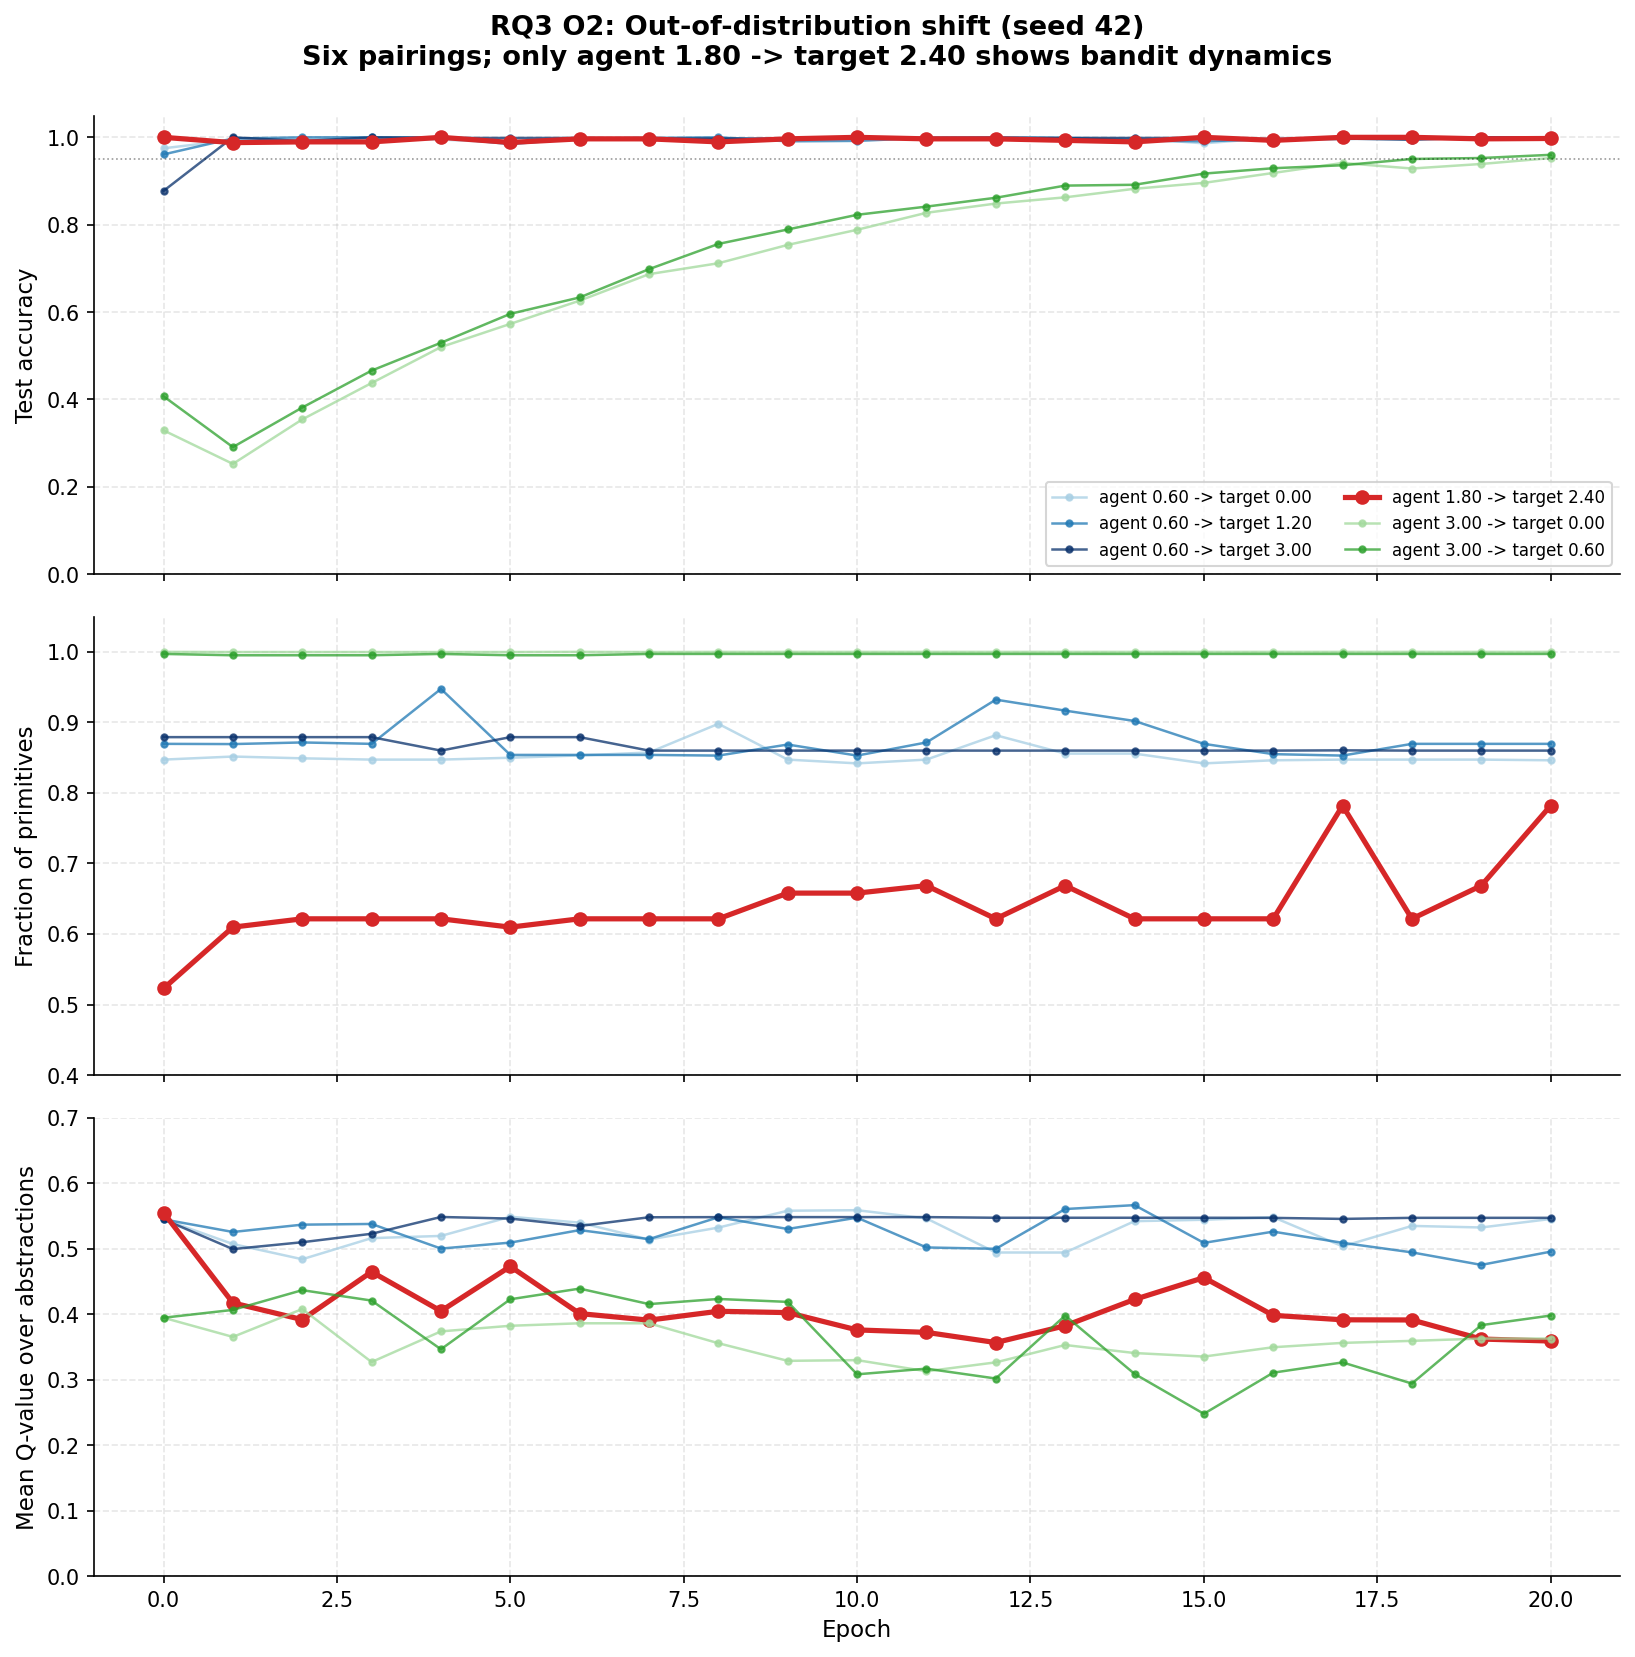
\includegraphics[width=0.95\textwidth]{images/rq3_o2_overview.png}}{\missingfigure{images/rq3_o2_overview.png}}
    \caption{Out-of-distribution shift dynamics, with agent $1.80 \rightarrow$ target $2.40$ highlighted as the only pairing with substantial bandit dynamics.}
    \label{fig:rq3-o2-overview}
\end{figure}

The out-of-distribution setup takes a single trained agent, uses the same checkpoint as both speaker and listener, and moves it to a distributional environment it never saw during its own training. Because speaker and listener are literally the same agent by construction, any change in behaviour has to be attributed to the distributional shift alone, not to a cross-population mismatch.

We tested six pairings. The results fall into three qualitatively distinct groups.

The sweep separates the agents by how much room their libraries leave for bandit-level change. Agents trained at $\alpha = 0.60$ already cover the shifted targets well: accuracy is high from epoch 0, primitive use stays stable, and Q-values barely move. Agents trained at $\alpha = 3.00$ face the opposite problem. Their initial accuracy is low and improves only gradually, while primitive use and Q-values remain essentially flat, so adaptation runs through neural retuning rather than symbolic reorganisation. The only substantial bandit dynamics appear in the intermediate case, agent $\alpha = 1.80$ tested on target $\alpha = 2.40$, where accuracy is already perfect but primitive use rises and mean Q-value declines over training.

The three groups reveal a specific condition for observing bandit dynamics under distributional shift. The agent's original library must be neither too broad (uniform case, no change needed) nor too narrow (concentrated case, no change possible). The intermediate case, with $\alpha = 1.80$ and a target that shifts moderately toward a more concentrated regime, is the only setup in this sweep where the bandit actually reorganises its selection during exposure to the new distribution.

\subsection{O3: Qualitative Analysis of the \texorpdfstring{$1.80 \rightarrow 2.40$}{1.80 to 2.40} Pairing}
\label{sec:rq3-o3}

The aggregate metric of Section~\ref{sec:rq3-o2} tells us that the bandit's use of abstractions changes on the ($1.80 \rightarrow 2.40$) pairing, but not how. To answer that, we reran the pairing with per-abstraction logging: at every epoch and for every one of the speaker's 21 tracker entries (2 primitives and 19 candidate abstractions), we count how many scenes the bandit routed through that entry.

\begin{figure}[htbp]
    \centering
    \IfFileExists{images/rq3_o3_gallery.png}{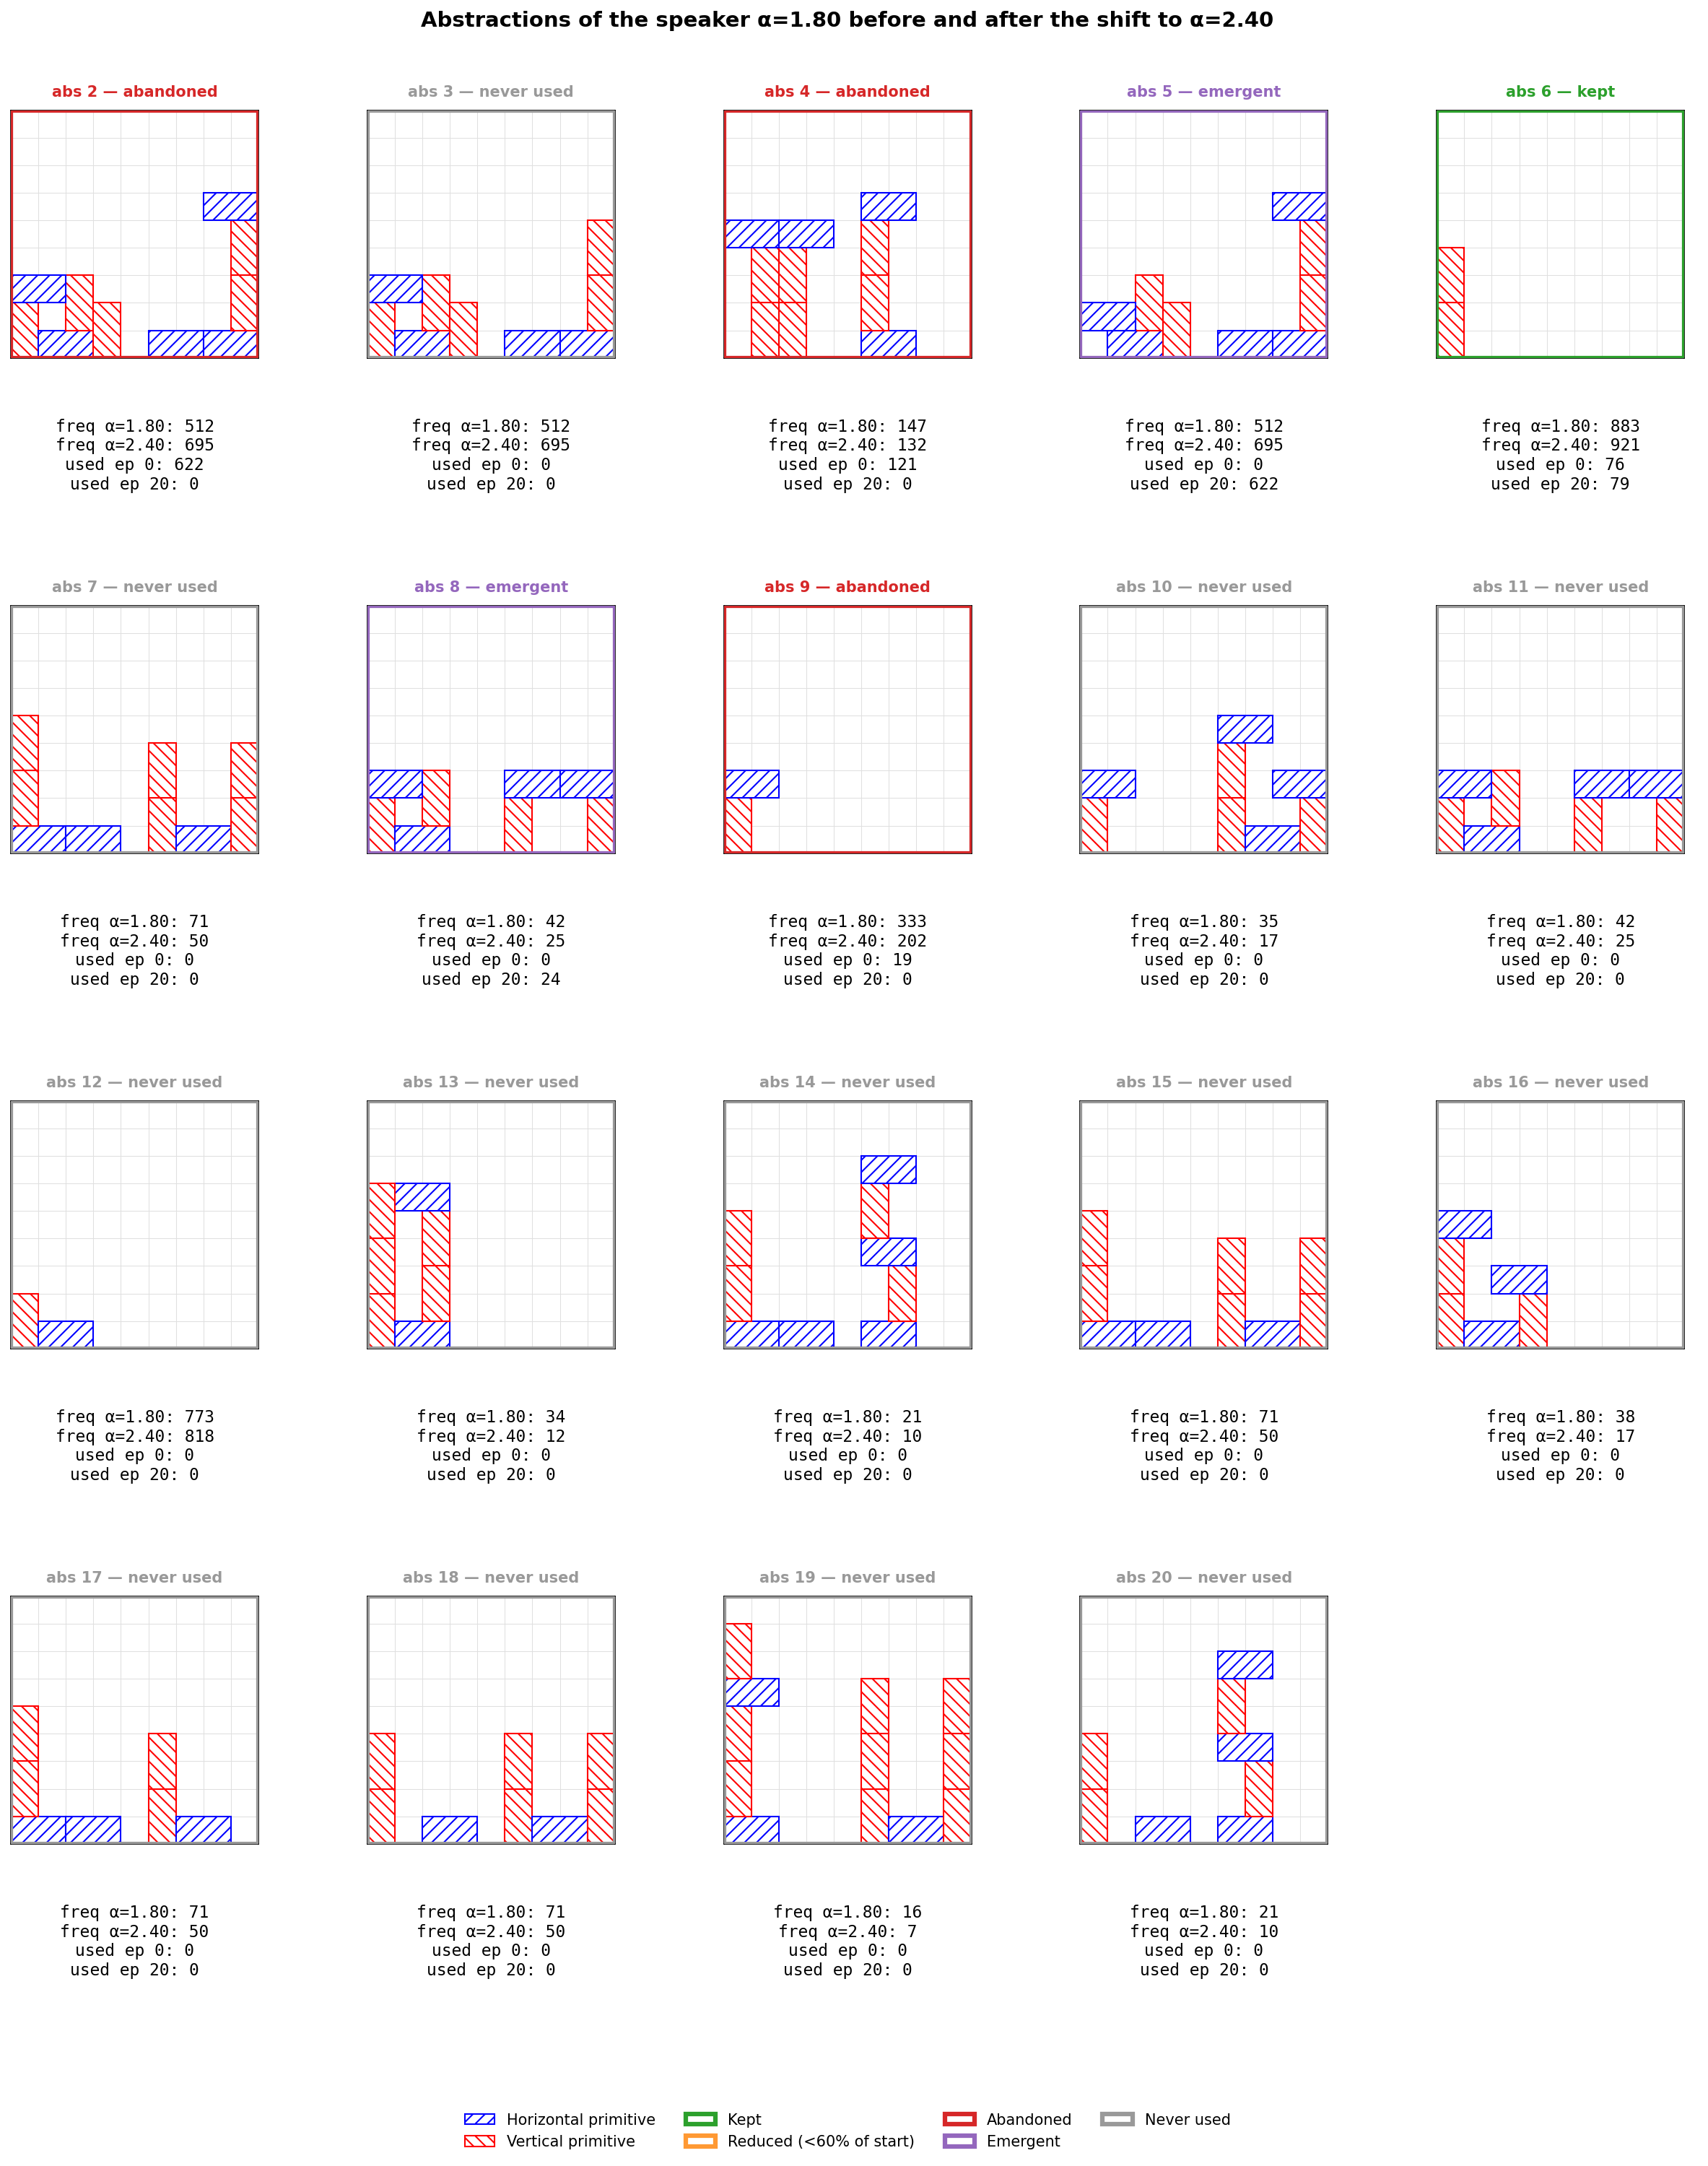
\includegraphics[width=0.95\textwidth]{images/rq3_o3_gallery.png}}{\missingfigure{images/rq3_o3_gallery.png}}
    \caption{Qualitative gallery for the $1.80 \rightarrow 2.40$ pairing. For each of the 19 candidate abstractions, the rendering is shown with its scene count at epoch 0 and epoch 20.}
    \label{fig:rq3-o3-gallery}
\end{figure}

The qualitative trace is best read as a single illustrative case rather than a population-level result. Within this one pairing, the bandit's response is structured rather than uniform and can be described through three sub-dynamics: substitution, abandonment, and emergence. Substitution occurs when two procedurally similar abstractions exchange roles while preserving the same structural motif; abandonment occurs when some abstractions fall out of use because they no longer match the shifted distribution; and emergence occurs when one previously dormant candidate becomes active. The exact counts are case-specific, but the conceptual point is important: symbolic adaptation can involve relabelling, dropping, and discovery at the same time. Because this analysis rests on seed 42 and the single $1.80 \rightarrow 2.40$ pairing, it should be treated as a hypothesis-generating example rather than as evidence that substitution is general.

\section{Discussion}
\label{sec:rq3-discussion}

\subsection{The Convergent Picture Across the Four Groups}
\label{sec:rq3-convergent-picture}

The four experimental groups combine into a coherent picture of cross-population and cross-distribution communication in PACE.

Same-$\alpha$ cross-pairing (Group C) shows that adaptation difficulty is regime-dependent: fast at low $\alpha$, slow at moderate $\alpha$, and infeasible in 20 epochs at high $\alpha$. Within a given $\alpha$, none of the three distance metrics we tested reliably discriminates listeners, although the Jaccard on adopted libraries shows a weak monotone effect at $\alpha = 1.80$.

The modifications (Group M) expose the mechanistic components of the same-$\alpha$ dynamics. When we give the bandit the option to bypass the speaker's abstractions (M1), a consistent unlearn-then-relearn dynamic on the mean Q-value emerges. Pretraining on primitives (M2) accelerates the neural side of adaptation without altering the symbolic side. Increased bandit exploration (M3) preserves more Q-value in the abstractions by giving them more opportunities to prove their usefulness.

Cross-$\alpha$ pairing (Group X) reveals a structural bottleneck that same-$\alpha$ pairing cannot detect. The bottleneck is asymmetric: concentrated speakers produce libraries that are too specialised to pair robustly with listeners from different regimes, while uniform speakers produce libraries that are broadly compatible. Comparing the frozen and unfrozen speaker settings shows that this gap is not neural: letting the speaker co-adapt does not close it.

The case studies (Group O) probe conditions further from the training setup. The mixed-distribution setup (O1) does not produce the expected unlearning dynamic, because the revert-to-primitives option structurally favours primitives when the listener does not initially understand the abstractions. The out-of-distribution shift (O2) reveals dynamics only in the narrow regime where the agent's library is neither too broad nor too narrow. The qualitative analysis of the one dynamics-showing pairing (O3) shows that when adaptation does happen at the symbolic level, it takes the form of three distinct sub-dynamics: substitution, abandonment, and emergence.

\subsection{What the Current Experiments Cannot Answer}
\label{sec:rq3-open-questions}

Our results support a coherent structural interpretation, but several questions stay open.

The Jaccard-on-libraries effect at $\alpha = 1.80$ (Section~\ref{sec:rq3-c-results}) is too small and too under-sampled to serve as a definitive statement about the role of library overlap in cross-pairing adaptation. A stronger test would need either many more seeds per condition, or a setup that removes the fast neural adaptation from the picture, for example, by freezing the listener and comparing epoch-0 accuracies across many cross-pairings.

The cross-$\alpha$ asymmetry (Section~\ref{sec:rq3-group-x}) is based on two speaker seeds and one seed for the listener at each configuration. Rotating the reference across all twenty speaker seeds would remove the dependence on the specific abstraction libraries of seeds 42 and 123.

The qualitative dynamics of Section~\ref{sec:rq3-o3} (substitution, abandonment, emergence) are based on a single pairing and a single seed. Replicating on other pairings and seeds would clarify whether the substitution dynamic in particular is a general property of PACE or a specific feature of this seed's library.